\chapter{Backup}
\label{chap:Backup}

\section{Dilepton Plots with \mediumPP\ Electrons}
\graphicspath{{Chapters/ObjEventSelection/Figures/}}

\begin{figure}[h]
\centering
	\subfigure[7~\tev]{
            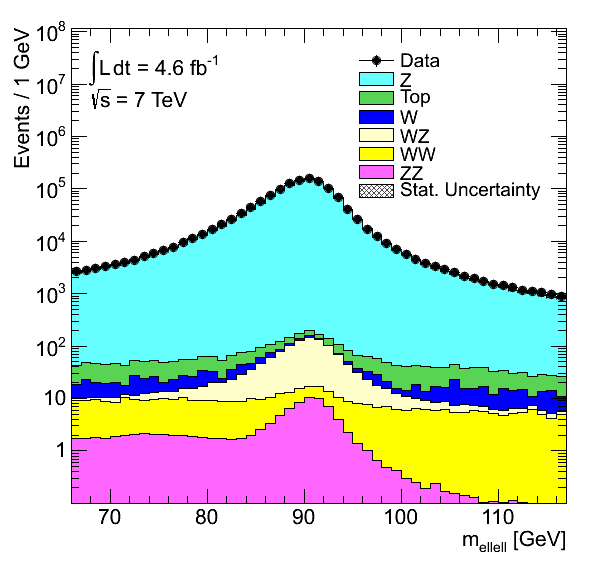
\includegraphics[width=0.47\textwidth]{Dilepton7TeV/CeECeE_pt20MediumPP_Z_m}
        }
	\subfigure[8~\tev]{
            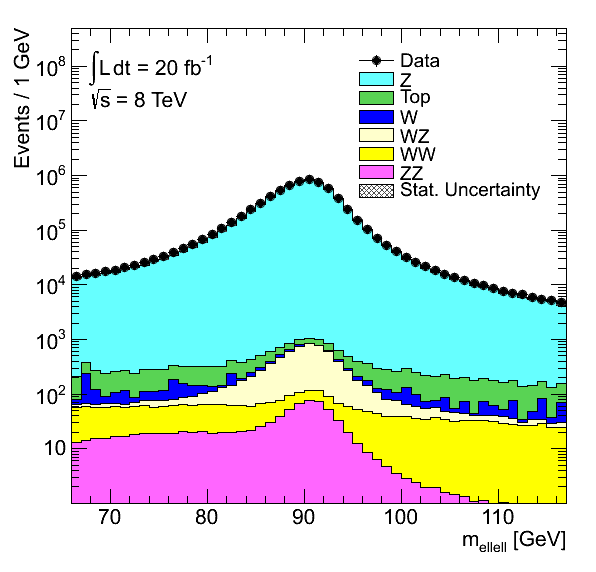
\includegraphics[width=0.47\textwidth]{Dilepton8TeV/CeECeE_pt20MediumPP_Z_m}
        }
	\subfigure[7~\tev]{
            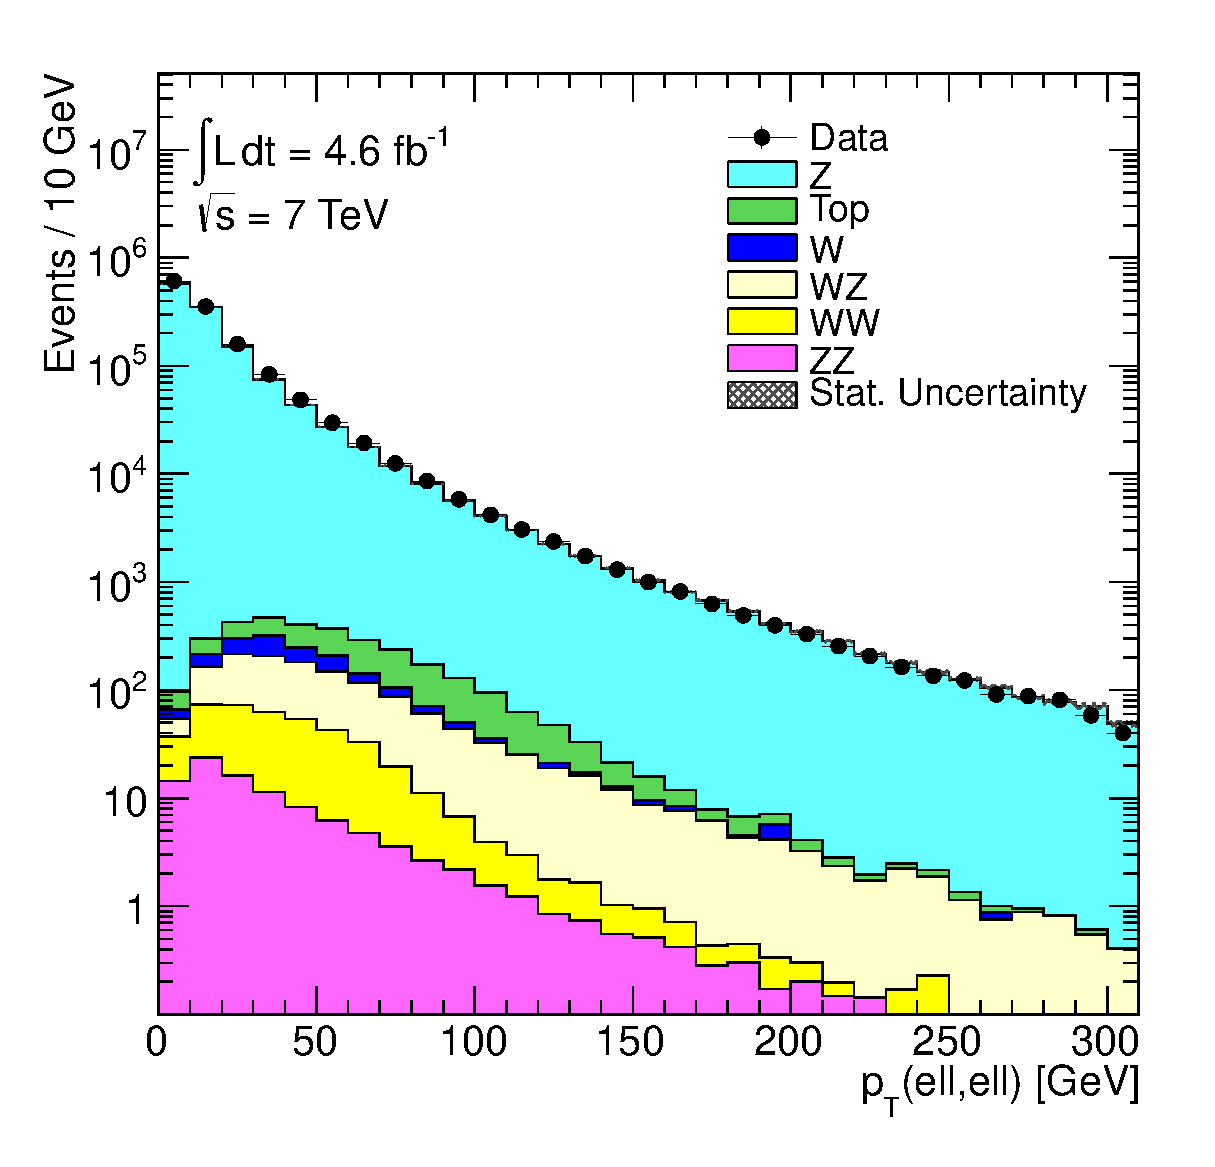
\includegraphics[width=0.47\textwidth]{Dilepton7TeV/CeECeE_pt20MediumPP_Z_pt}
        }
	\subfigure[8~\tev]{
            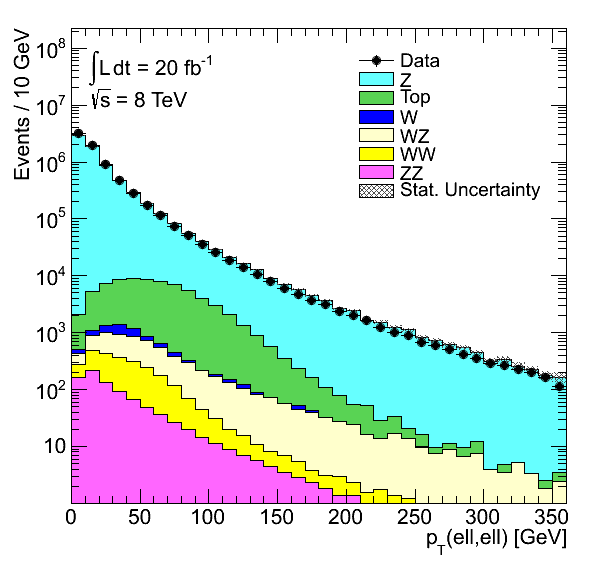
\includegraphics[width=0.47\textwidth]{Dilepton8TeV/CeECeE_pt20MediumPP_Z_pt}
        }
    \caption[Dilepton invariant mass and transverse momentum in the 7~\tev\
    data. ]
    {Kinematic distributions for
    \dielectron\ pairs, for the 7~\tev\ and the 8~\tev\ data respectively, in events containing a pair of
    \ossf\ electrons with the electron selection tightened to require both
    electrons satisfy the \mediumPP\ requirements and have \ptgt{20}. 
    }
\label{fig:dilep-mass-pt-seven}
\end{figure}

\begin{figure}[h]
\centering
\vspace{-5mm}
	\subfigure[7~\tev]{
            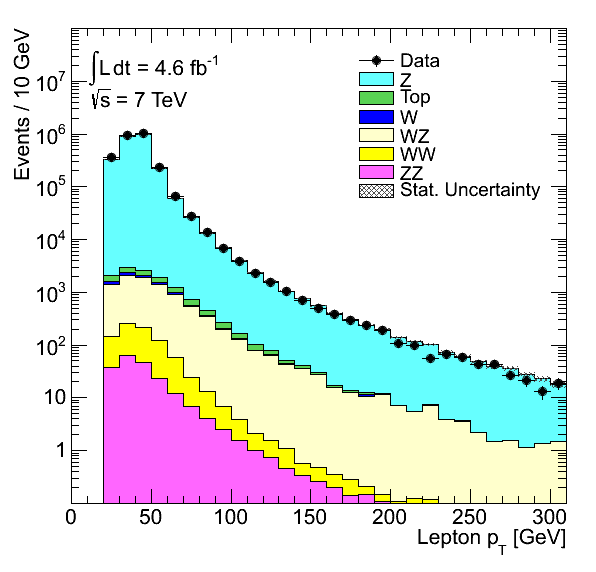
\includegraphics[width=0.47\textwidth]{Dilepton7TeV/CeECeE_pt20MediumPP_lep_pt}
        }
	\subfigure[8~\tev]{
            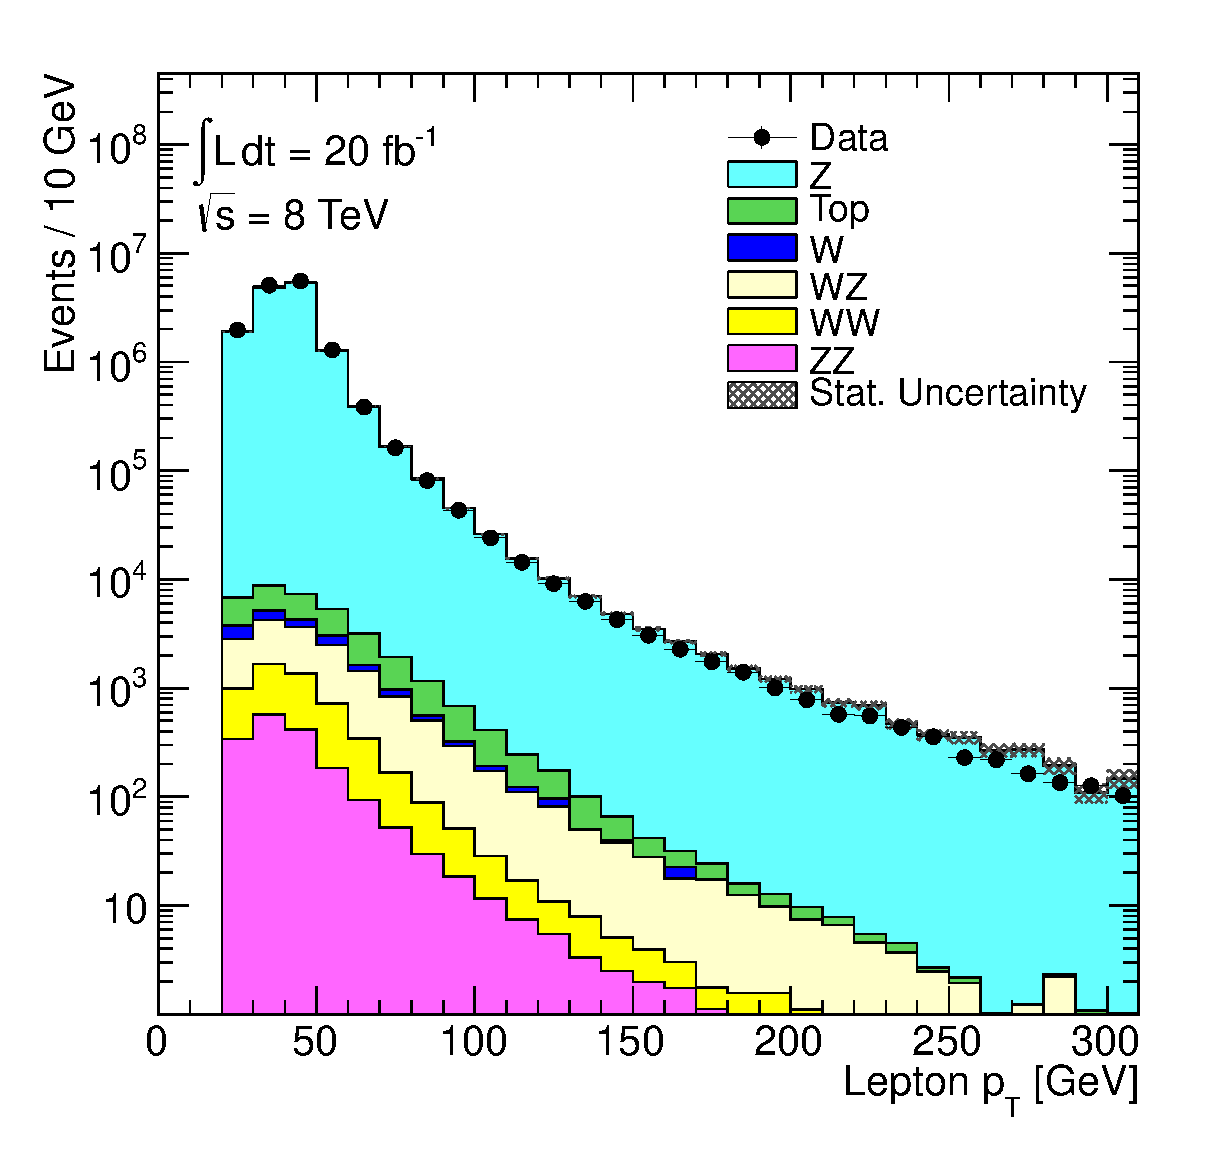
\includegraphics[width=0.47\textwidth]{Dilepton8TeV/CeECeE_pt20MediumPP_lep_pt}
        }
	\subfigure[7~\tev]{
            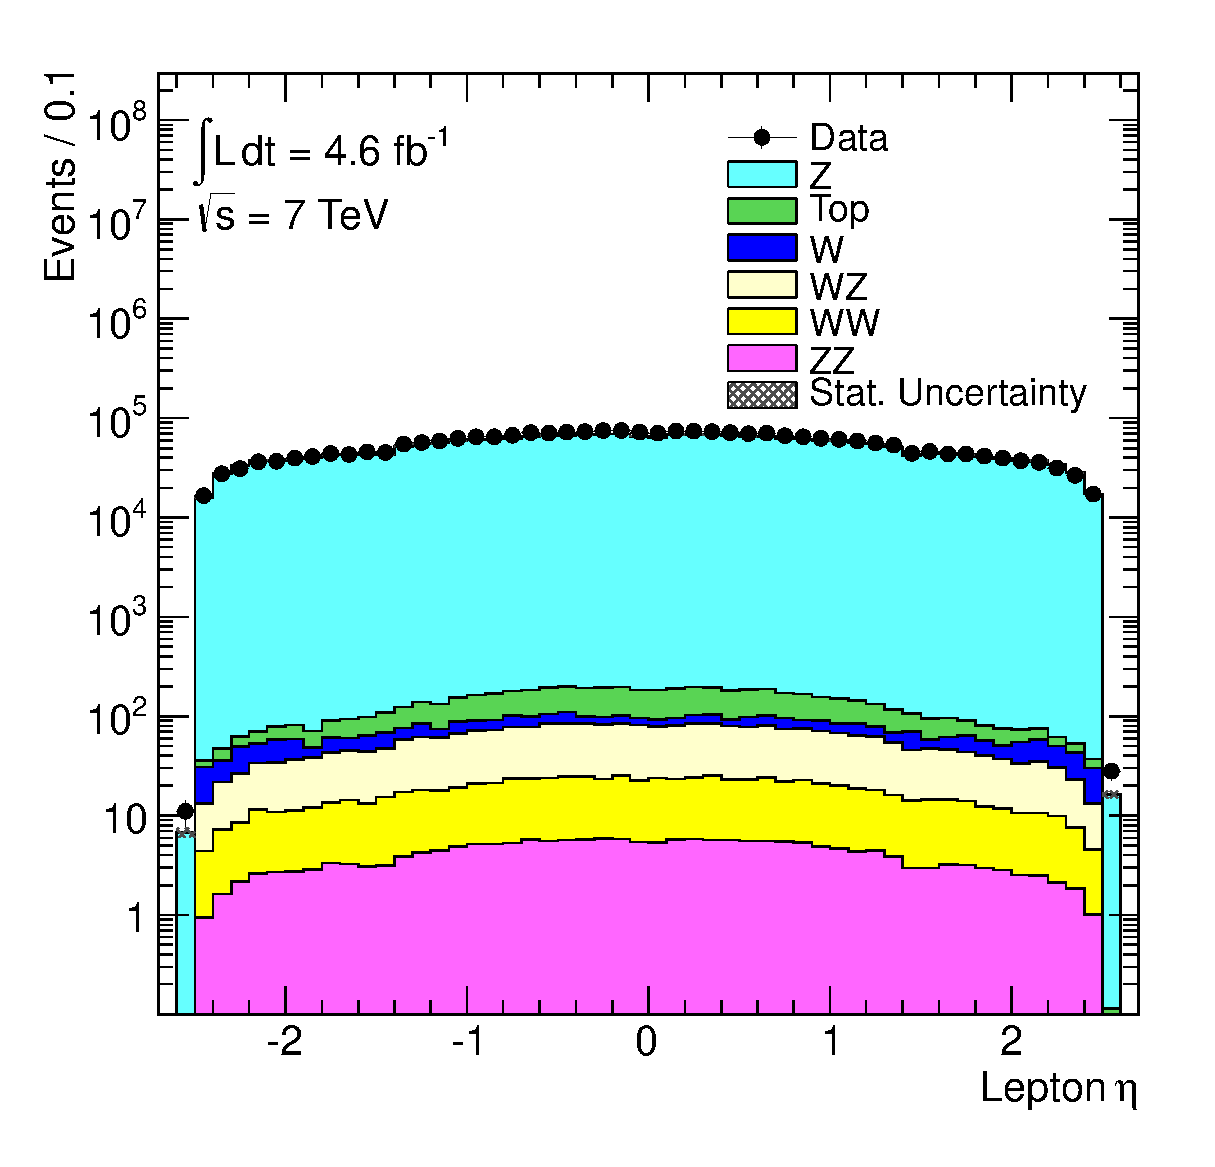
\includegraphics[width=0.47\textwidth]{Dilepton7TeV/CeECeE_pt20MediumPP_lep_eta}
        }
	\subfigure[8~\tev]{
            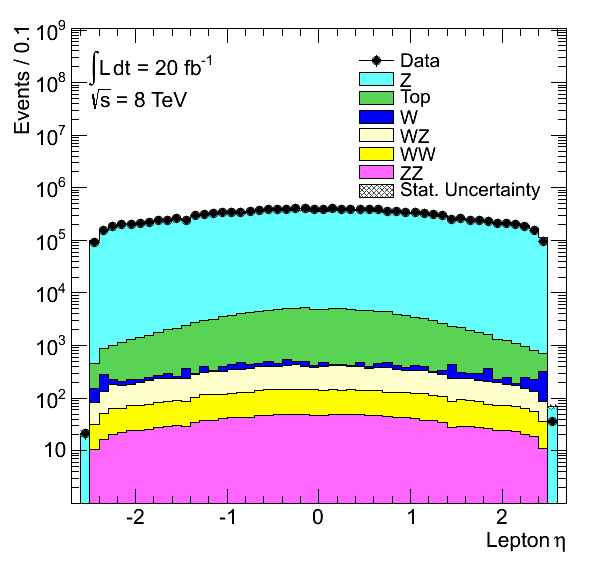
\includegraphics[width=0.47\textwidth]{Dilepton8TeV/CeECeE_pt20MediumPP_lep_eta}
        }
	\subfigure[7~\tev]{
            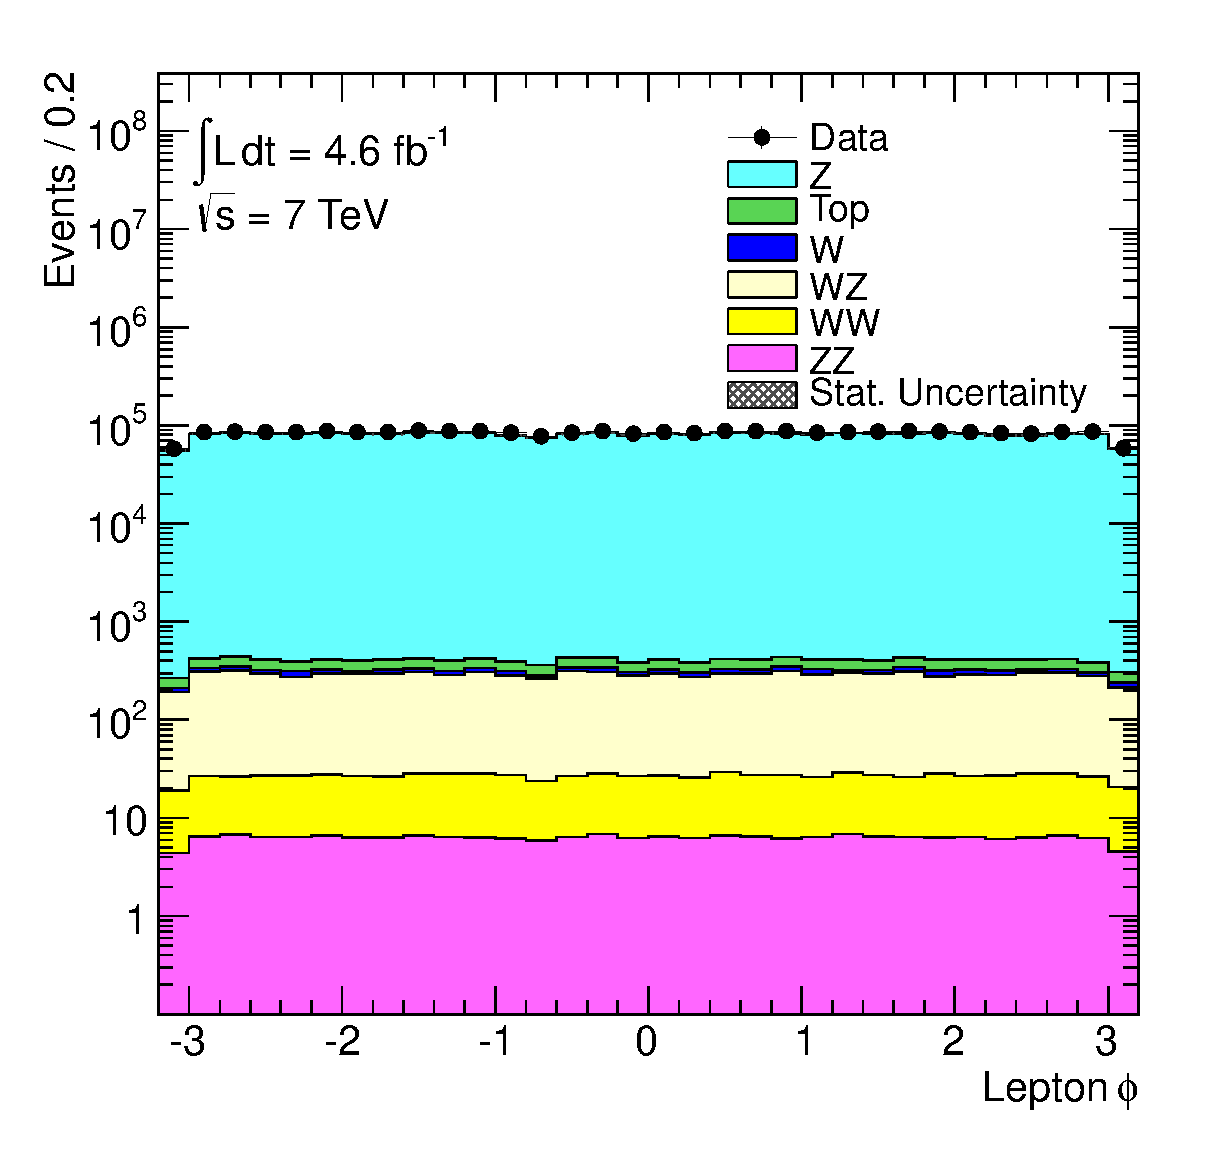
\includegraphics[width=0.47\textwidth]{Dilepton7TeV/CeECeE_pt20MediumPP_lep_phi}
        }
	\subfigure[8~\tev]{
            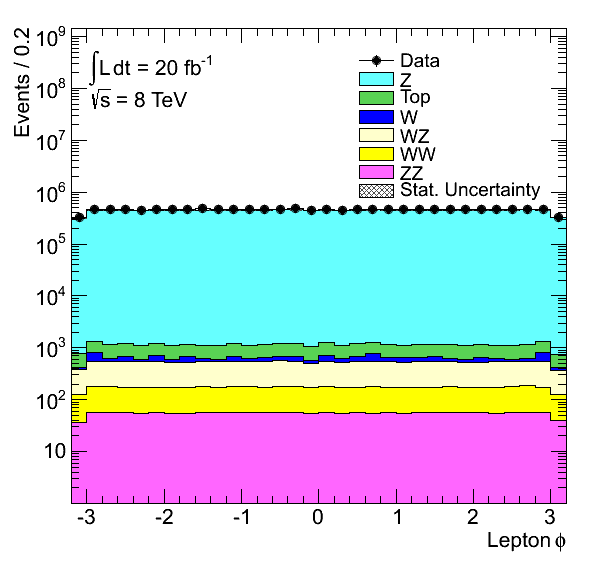
\includegraphics[width=0.47\textwidth]{Dilepton8TeV/CeECeE_pt20MediumPP_lep_phi}
        }
    \caption[Lepton kinematic distributions for \dilep\ events in the 7~\tev\
    data. ]
    {\small Kinematic distributions for
    electron  in events containing a pair of
    \ossf\ electrons, with the electron selection tightened to require both
    electrons satisfy the \mediumPP\ requirements and have \ptgt{20}, for the 7~\tev\ and the 8~\tev\ data. }
\label{fig:dilep-lepkin-seven}
\end{figure}

\section{Plots with Ratios}
\graphicspath{{Chapters/Backup/Figures/}}

\begin{figure}[h]
\centering
	\subfigure[]{
            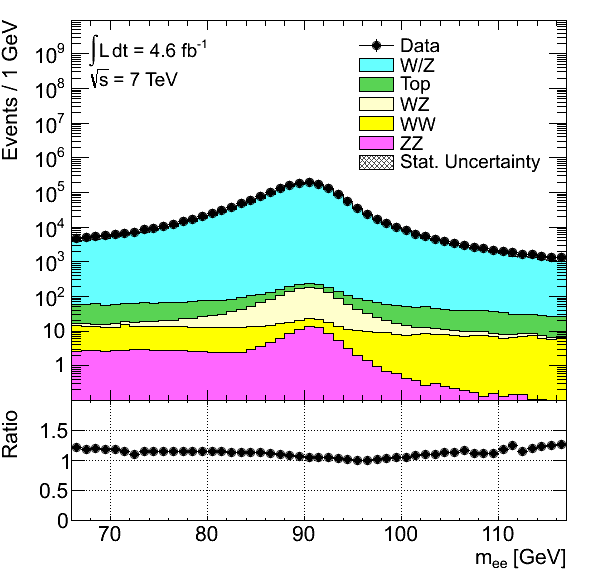
\includegraphics[width=0.47\textwidth]{Dilepton7TeVRatio/AllE_Z_m}
        }
	\subfigure[]{
            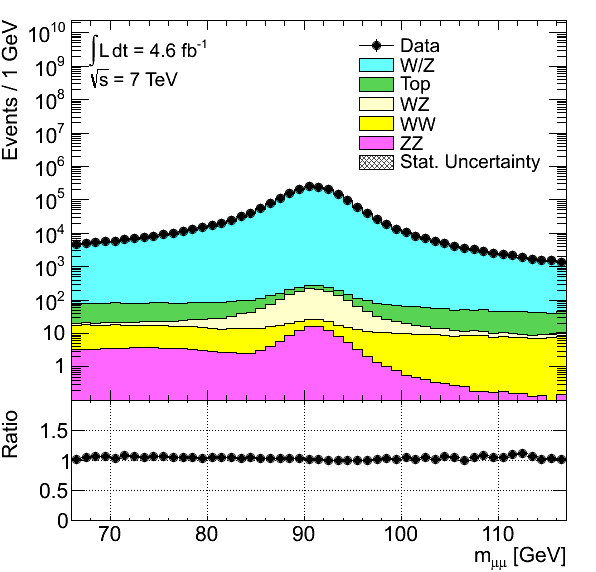
\includegraphics[width=0.47\textwidth]{Dilepton7TeVRatio/AllMu_Z_m}
        }
	\subfigure[]{
            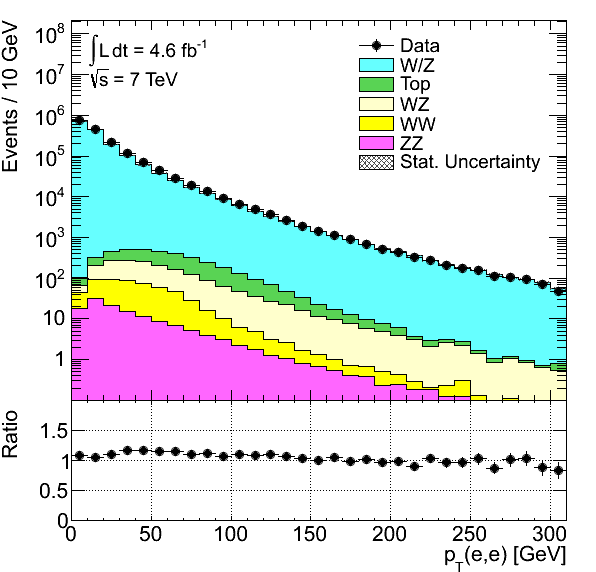
\includegraphics[width=0.47\textwidth]{Dilepton7TeVRatio/AllE_Z_pt}
        }
	\subfigure[]{
            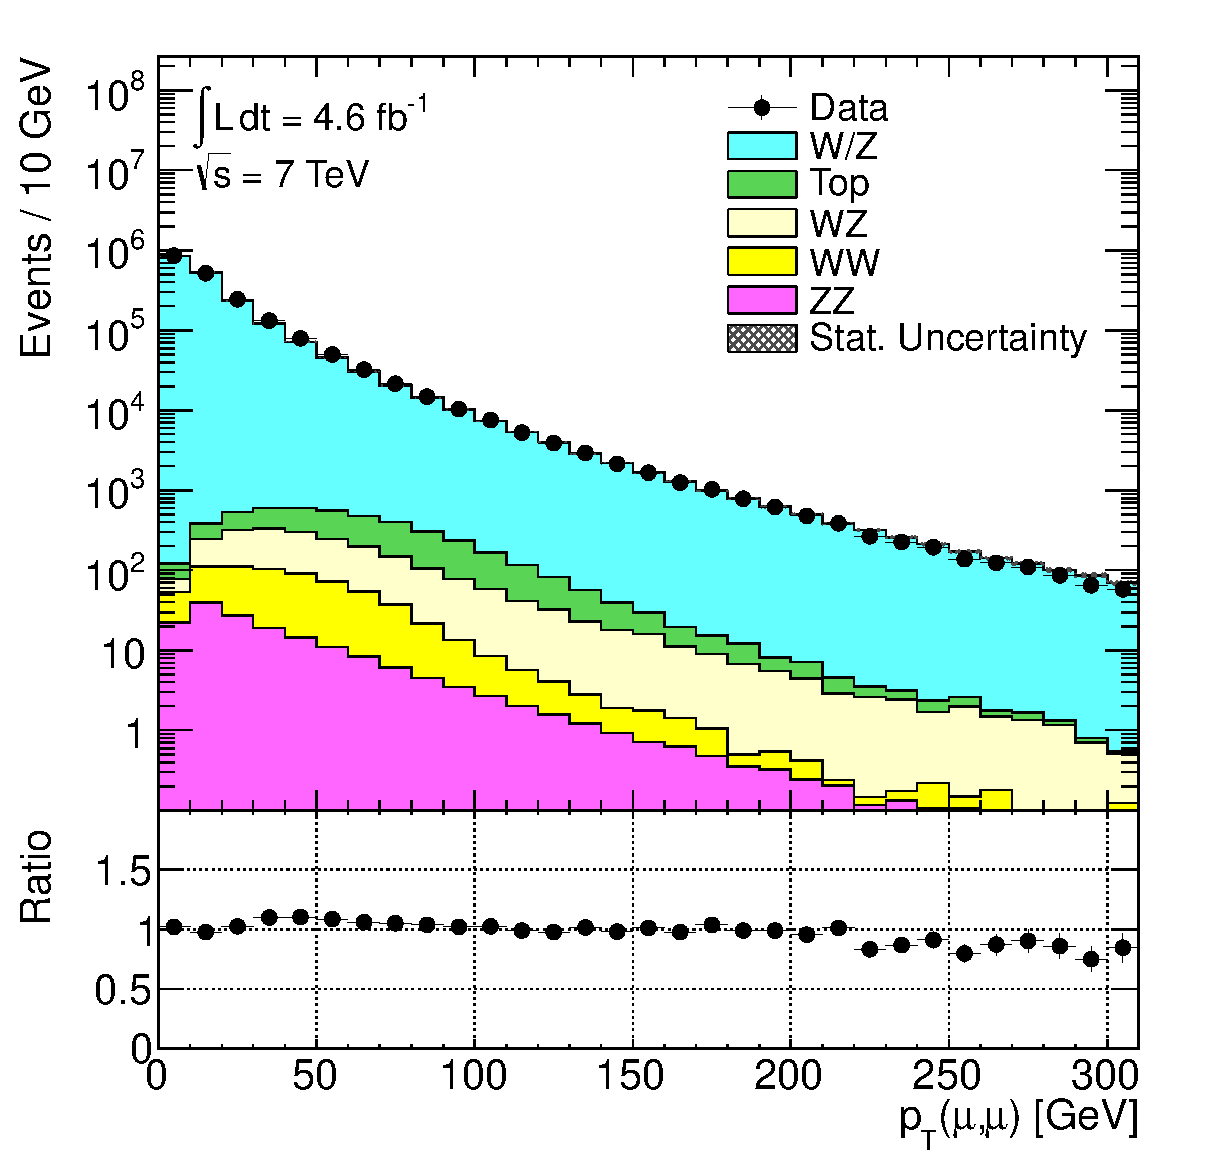
\includegraphics[width=0.47\textwidth]{Dilepton7TeVRatio/AllMu_Z_pt}
        }
    \caption[Dilepton invariant mass and transverse momentum in the 7~\tev\
    data. ]
    {Figures (a) and (b) show distributions of the \dilepton\ invariant mass for \dielectron\ and 
     \dimuon\ pairs, respectively, in events in the 7~\tev\ data containing a pair of
    \ossf\ leptons passing all of the lepton selection criteria described
    in Sections~\ref{sec:objsel-el} and~\ref{sec:objsel-mu}. Figures (c) and (d) show the \dilepton\ transverse momentum for
    events passing the same criteria, with the additional requirement that the
    \dilepton\ pair have \sstooos. 
    }
\label{fig:dilep-mass-pt-seven}
\end{figure}

\begin{figure}[h]
\centering
	\subfigure[]{
            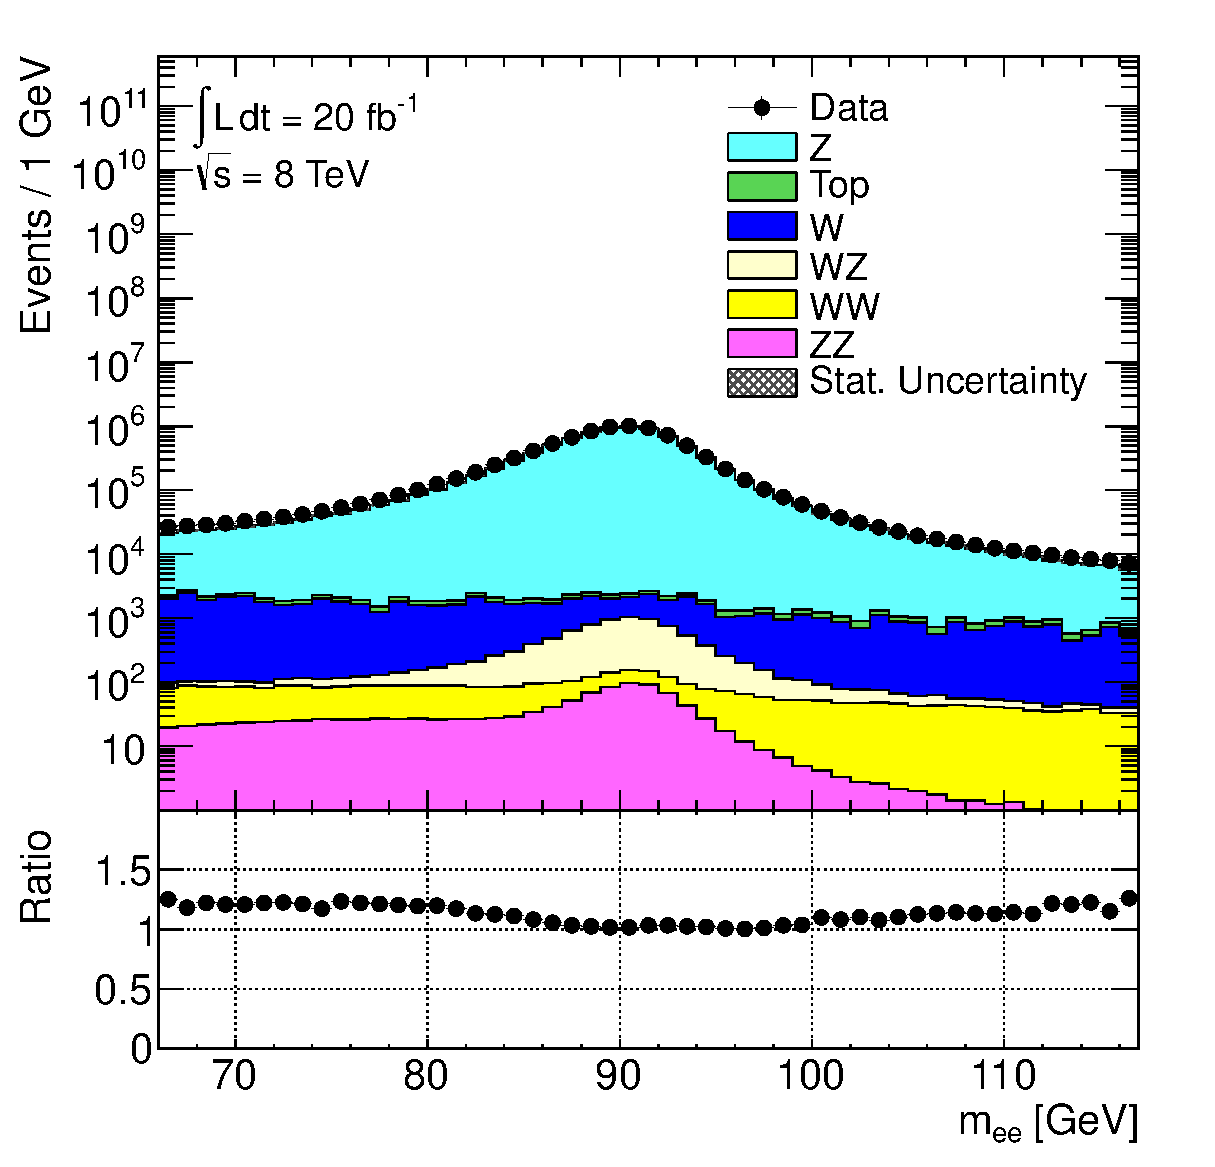
\includegraphics[width=0.47\textwidth]{Dilepton8TeVRatio/AllE_Z_m}
        }
	\subfigure[]{
            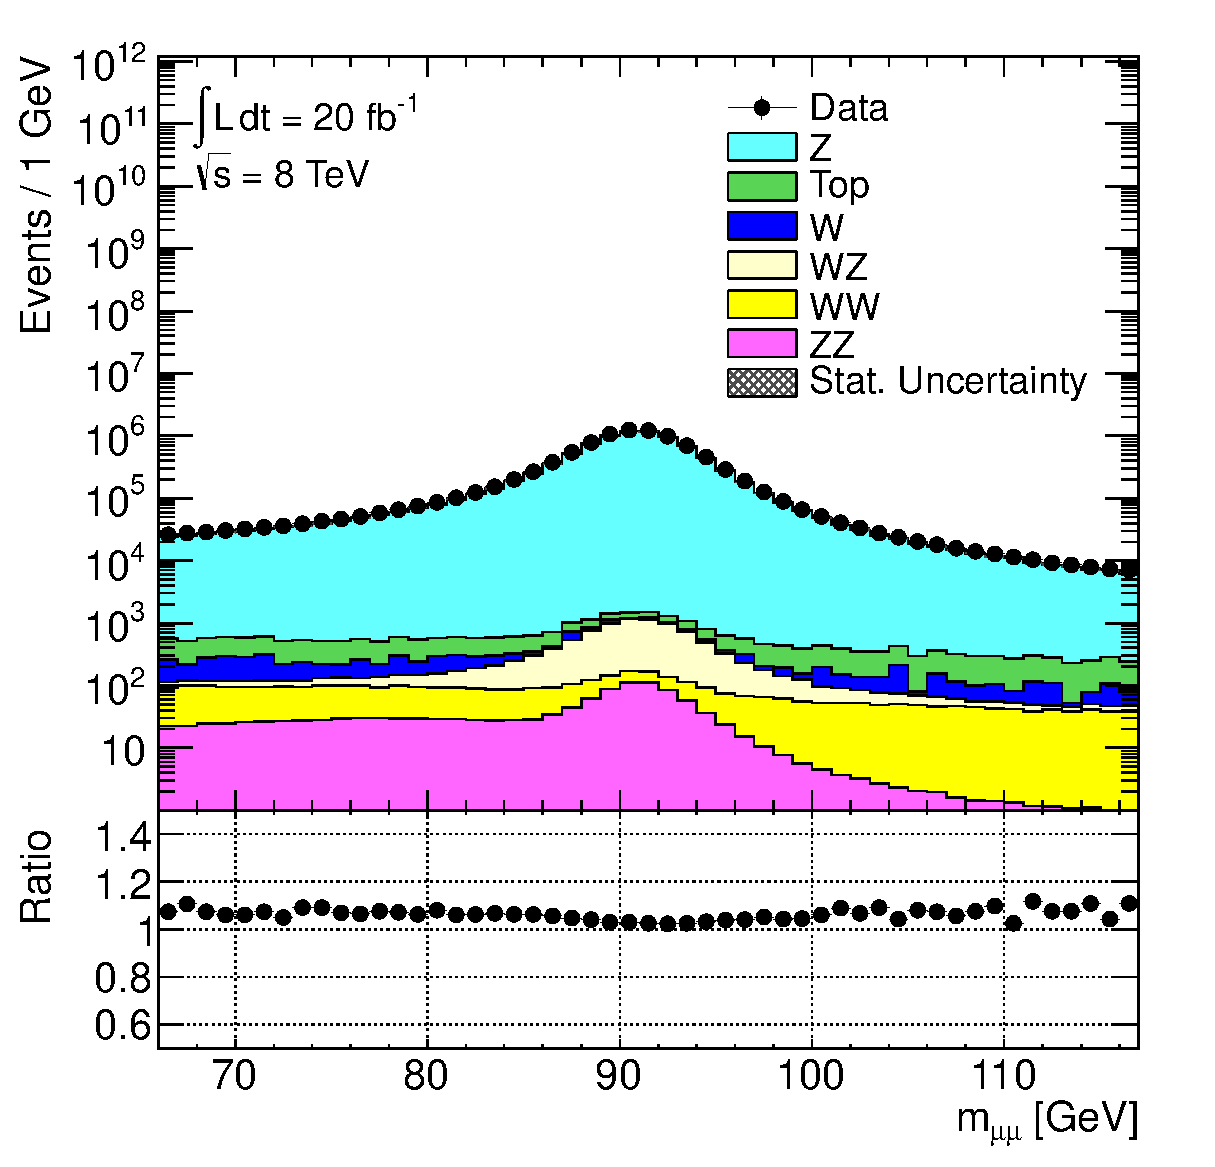
\includegraphics[width=0.47\textwidth]{Dilepton8TeVRatio/AllMu_Z_m}
        }
	\subfigure[]{
            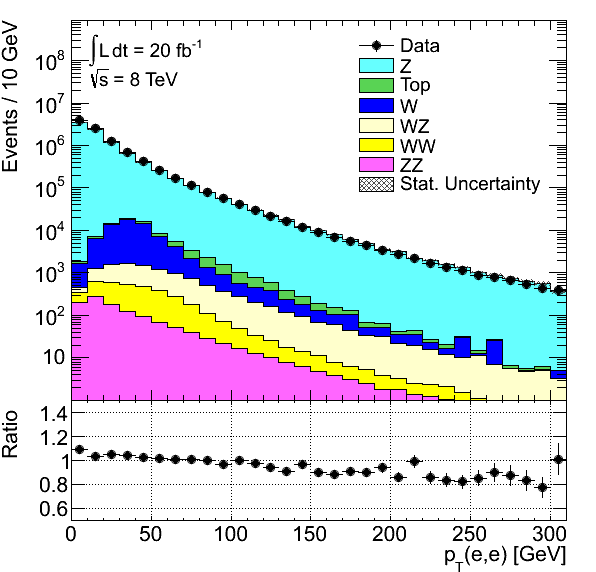
\includegraphics[width=0.47\textwidth]{Dilepton8TeVRatio/AllE_Z_pt}
        }
	\subfigure[]{
            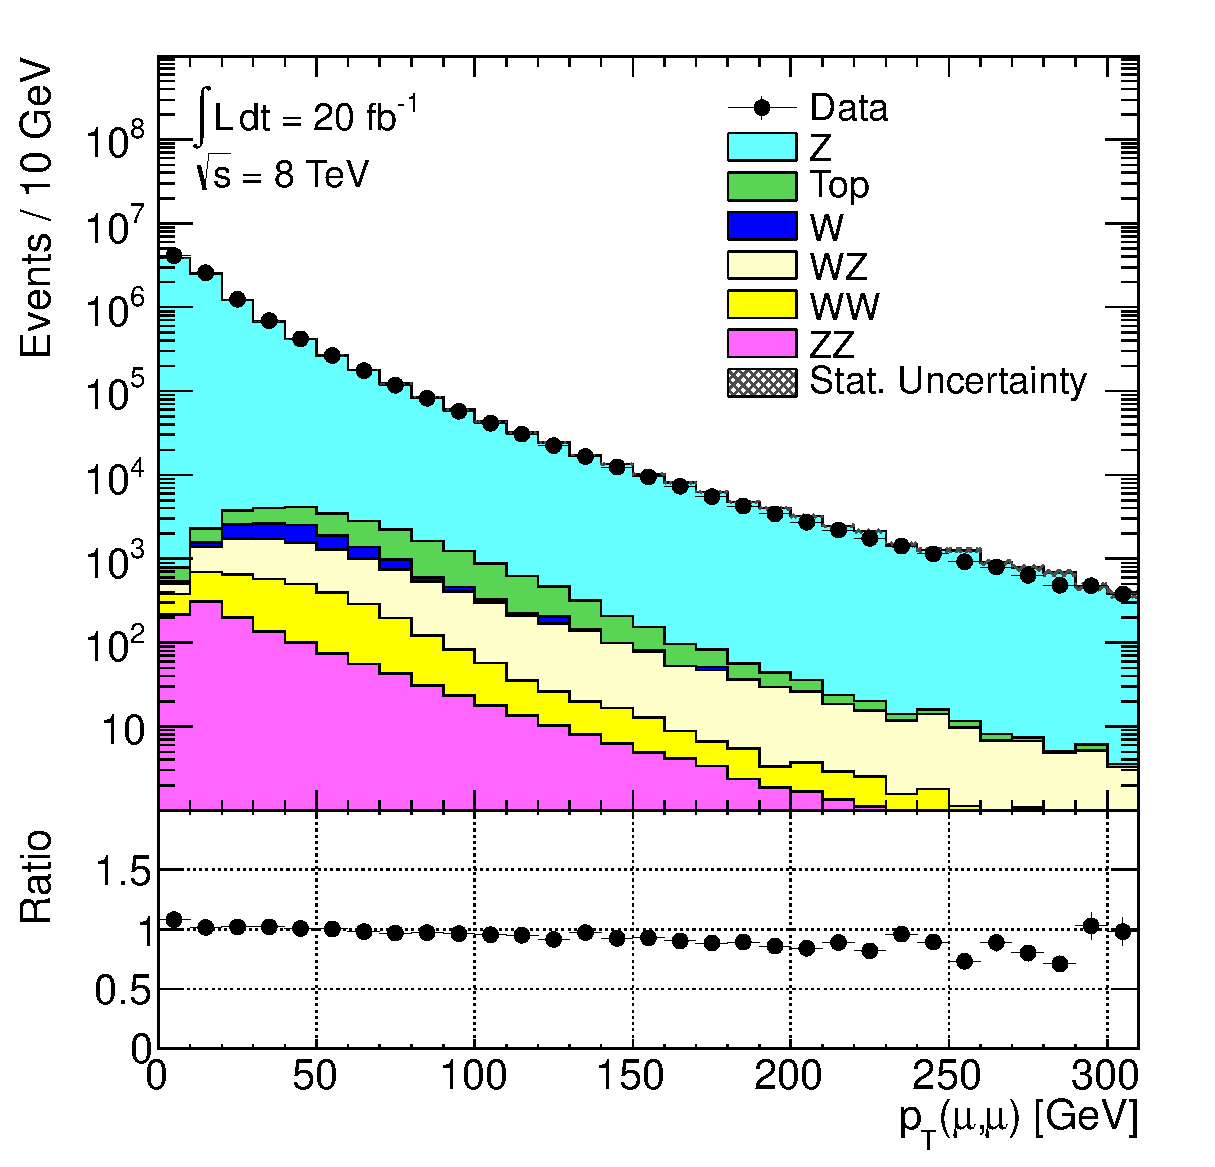
\includegraphics[width=0.47\textwidth]{Dilepton8TeVRatio/AllMu_Z_pt}
        }
    \caption[Dilepton invariant mass and transverse momentum in the 8~\tev\
    data. ]
    {Figures (a) and (b) show distributions of the \dilepton\ invariant mass for \dielectron\ and 
     \dimuon\ pairs, respectively, in events in the 8~\tev\ data containing a pair of
    \ossf\ leptons passing all of the lepton selection criteria described
    in Sections~\ref{sec:objsel-el} and~\ref{sec:objsel-mu}. Figures (c) and (d) show the \dilepton\ transverse momentum for
    events passing the same criteria, with the additional requirement that the
    \dilepton\ pair have \sstooos. 
    }
\label{fig:dilep-mass-pt-eight}
\end{figure}

\begin{figure}[h]
\centering
\vspace{-5mm}
	\subfigure[]{
            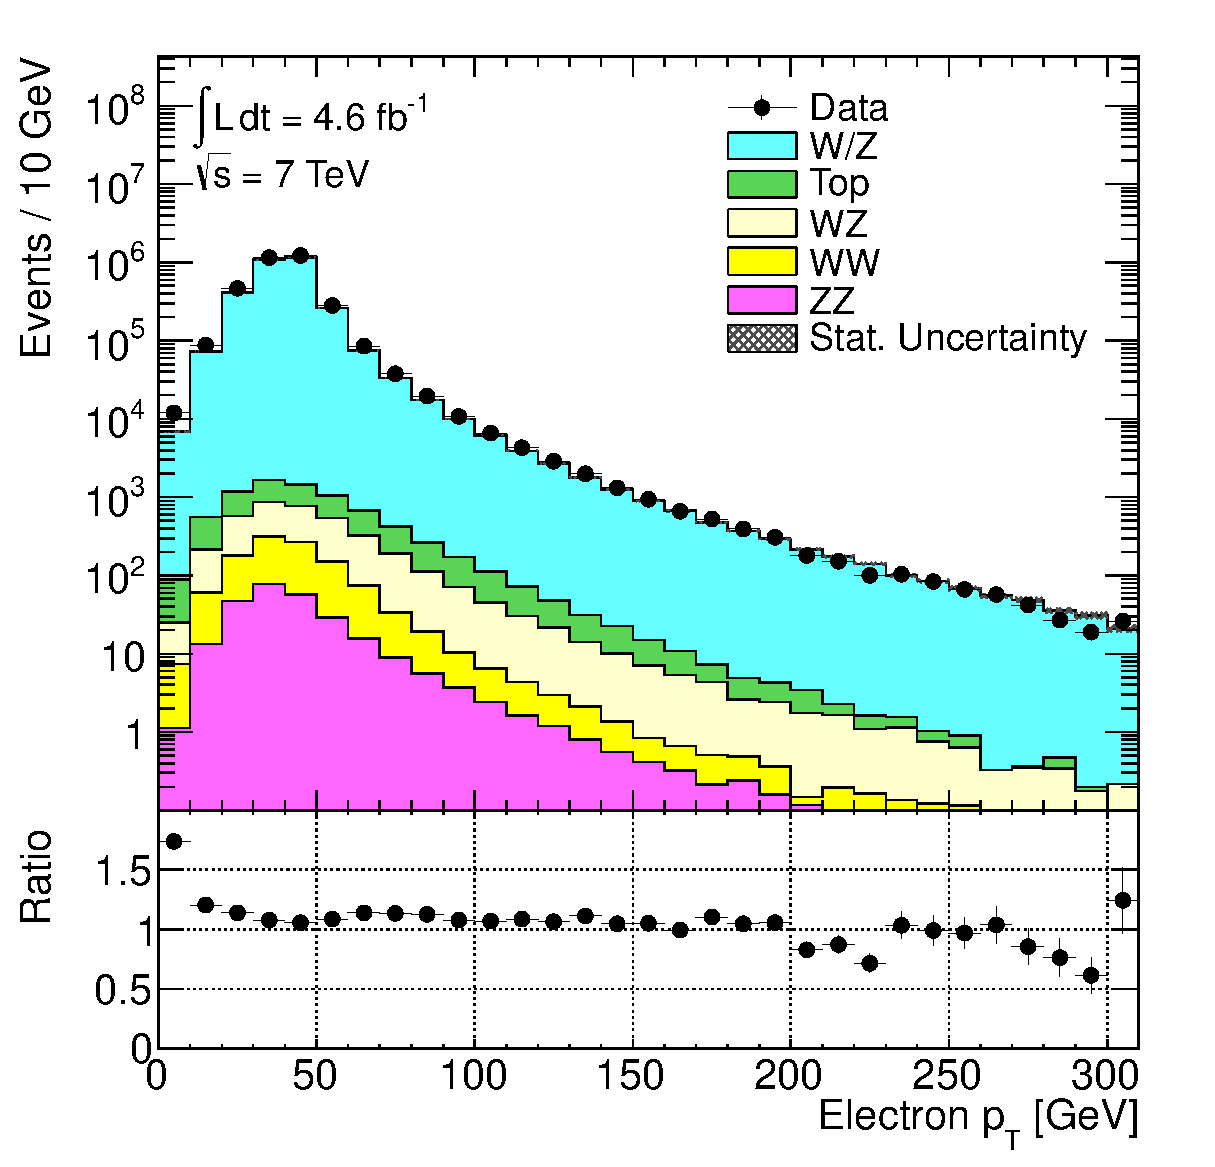
\includegraphics[width=0.47\textwidth]{Dilepton7TeVRatio/AllE_lep_pt}
        }
	\subfigure[]{
            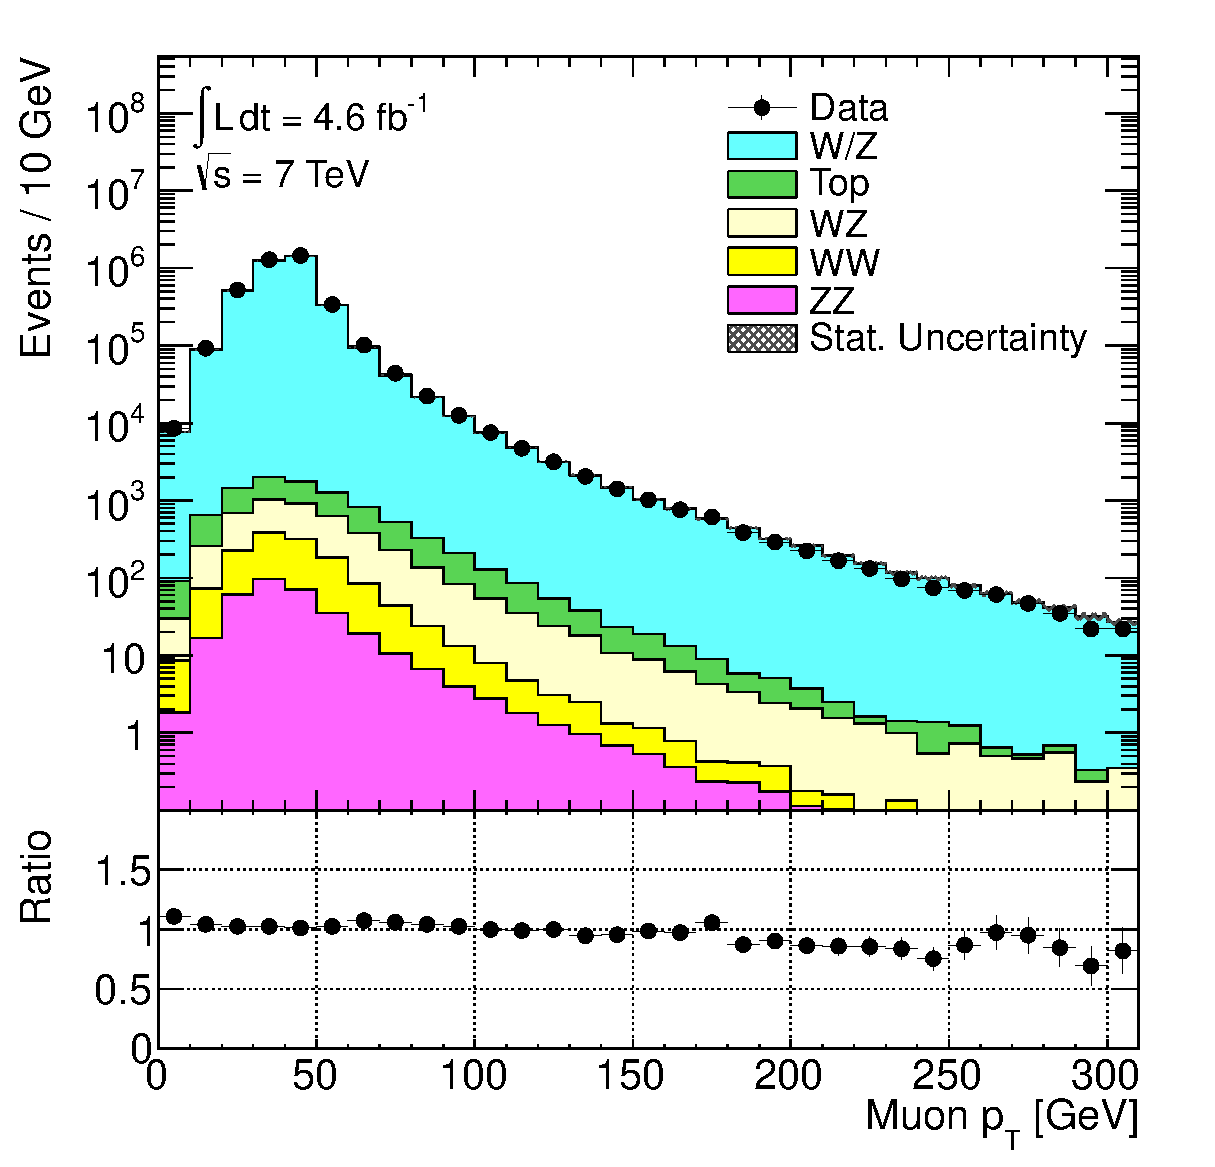
\includegraphics[width=0.47\textwidth]{Dilepton7TeVRatio/AllMu_lep_pt}
        }
	\subfigure[]{
            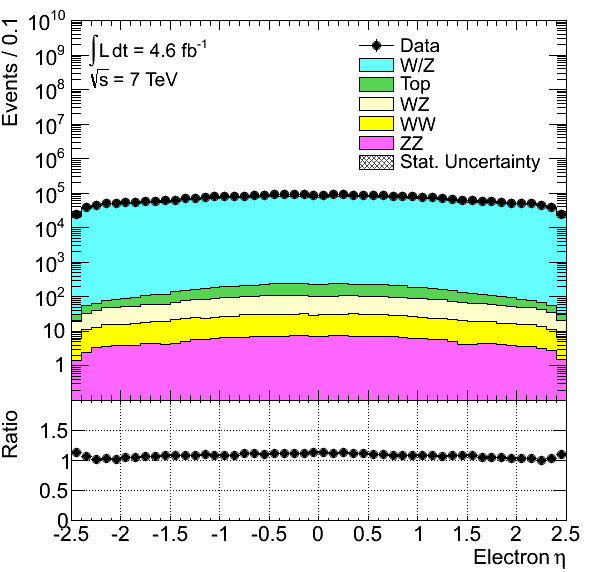
\includegraphics[width=0.47\textwidth]{Dilepton7TeVRatio/AllE_lep_eta}
        }
	\subfigure[]{
            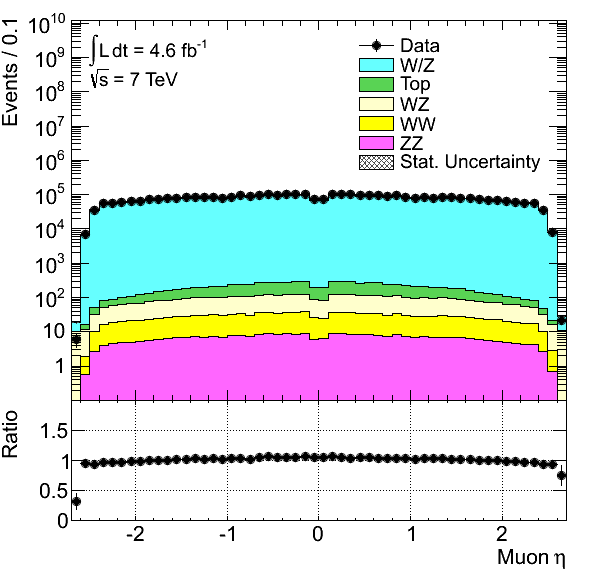
\includegraphics[width=0.47\textwidth]{Dilepton7TeVRatio/AllMu_lep_eta}
        }
	\subfigure[]{
            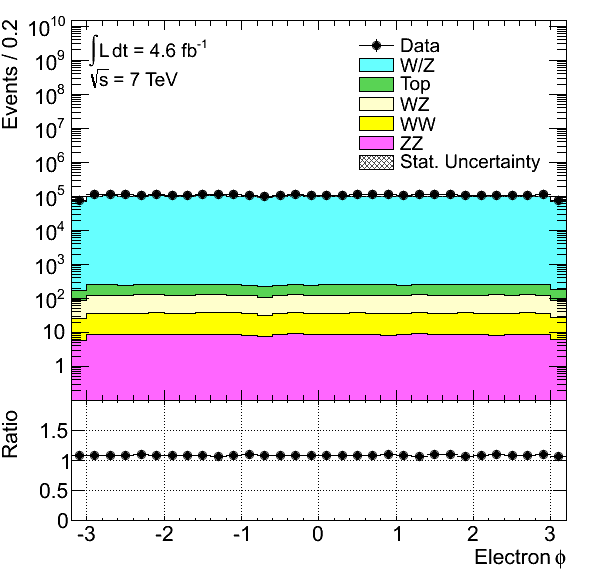
\includegraphics[width=0.47\textwidth]{Dilepton7TeVRatio/AllE_lep_phi}
        }
	\subfigure[]{
            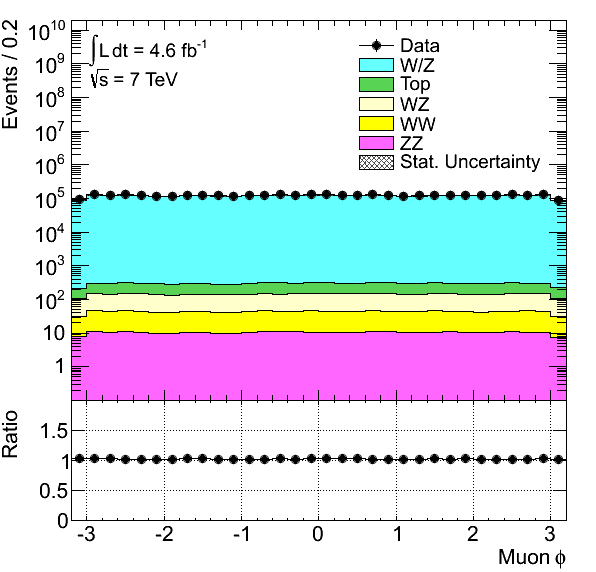
\includegraphics[width=0.47\textwidth]{Dilepton7TeVRatio/AllMu_lep_phi}
        }
    \caption[Lepton kinematic distributions for \dilep\ events in the 7~\tev\
    data. ]
    {\small Kinematic distributions for leptons in events in the 7~\tev\
    data containing an \ossf\ lepton pair. The leptons are required to pass all of the selection
    requirements described in Sections~\ref{sec:objsel-el}
    and~\ref{sec:objsel-mu} and the pair must have \sstooos. 
    Figures (a) and (b) show the lepton \pt\ for electrons and muons
    respectively, figures (c) and (d) the lepton $\eta$ and figures (d) and (e)
    the lepton $\phi$.    }
\label{fig:dilep-lepkin-seven}
\end{figure}

\begin{figure}[h]
\centering
\vspace{-5mm}
	\subfigure[]{
            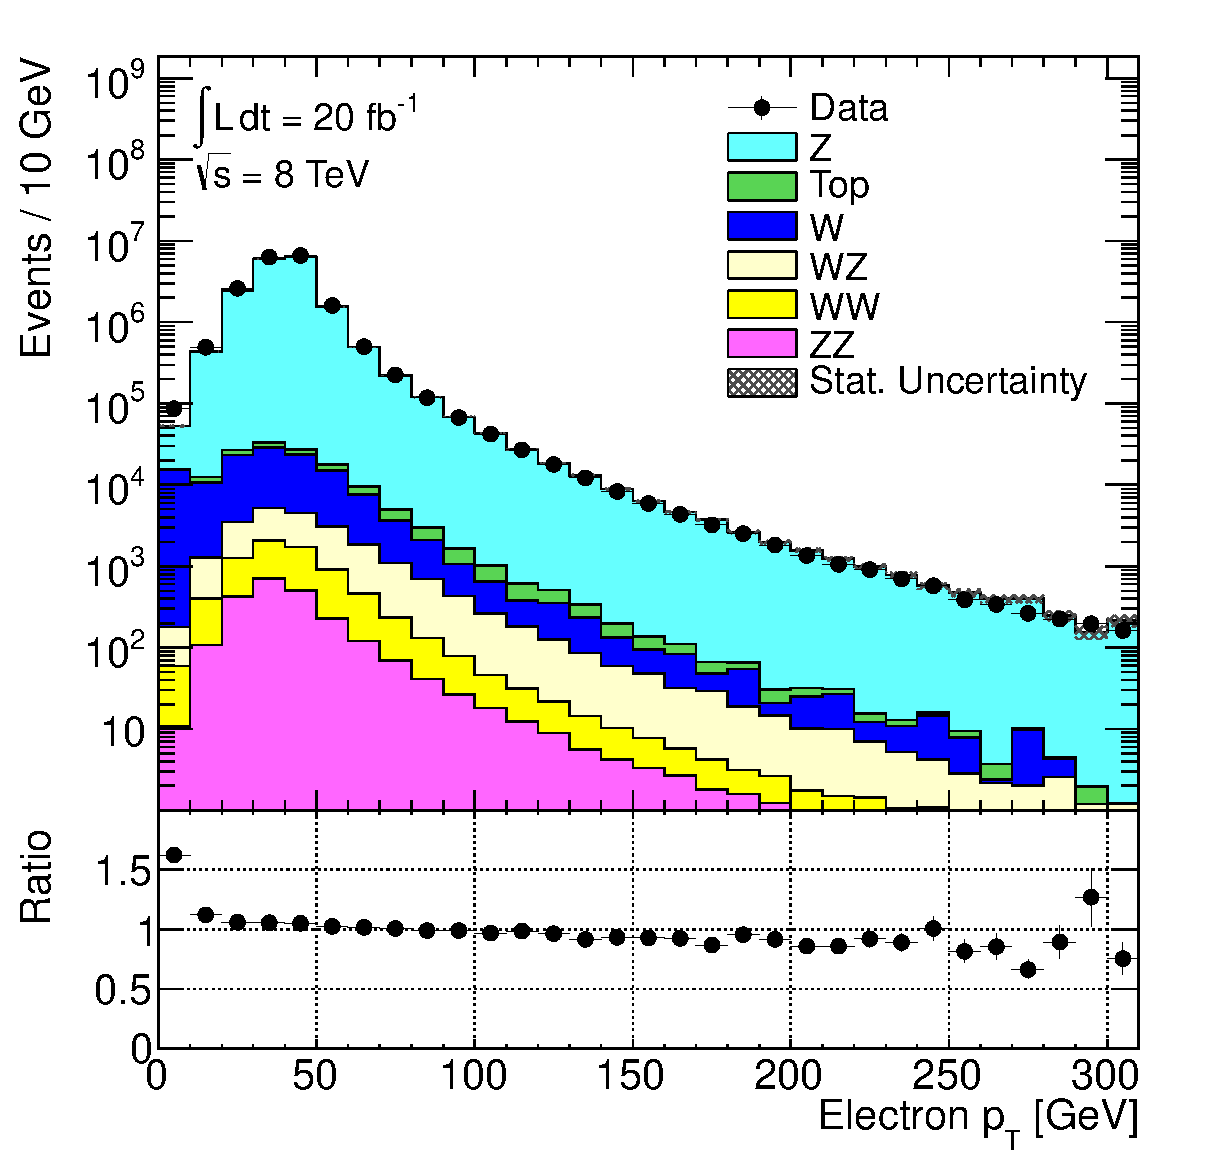
\includegraphics[width=0.47\textwidth]{Dilepton8TeVRatio/AllE_lep_pt}
        }
	\subfigure[]{
            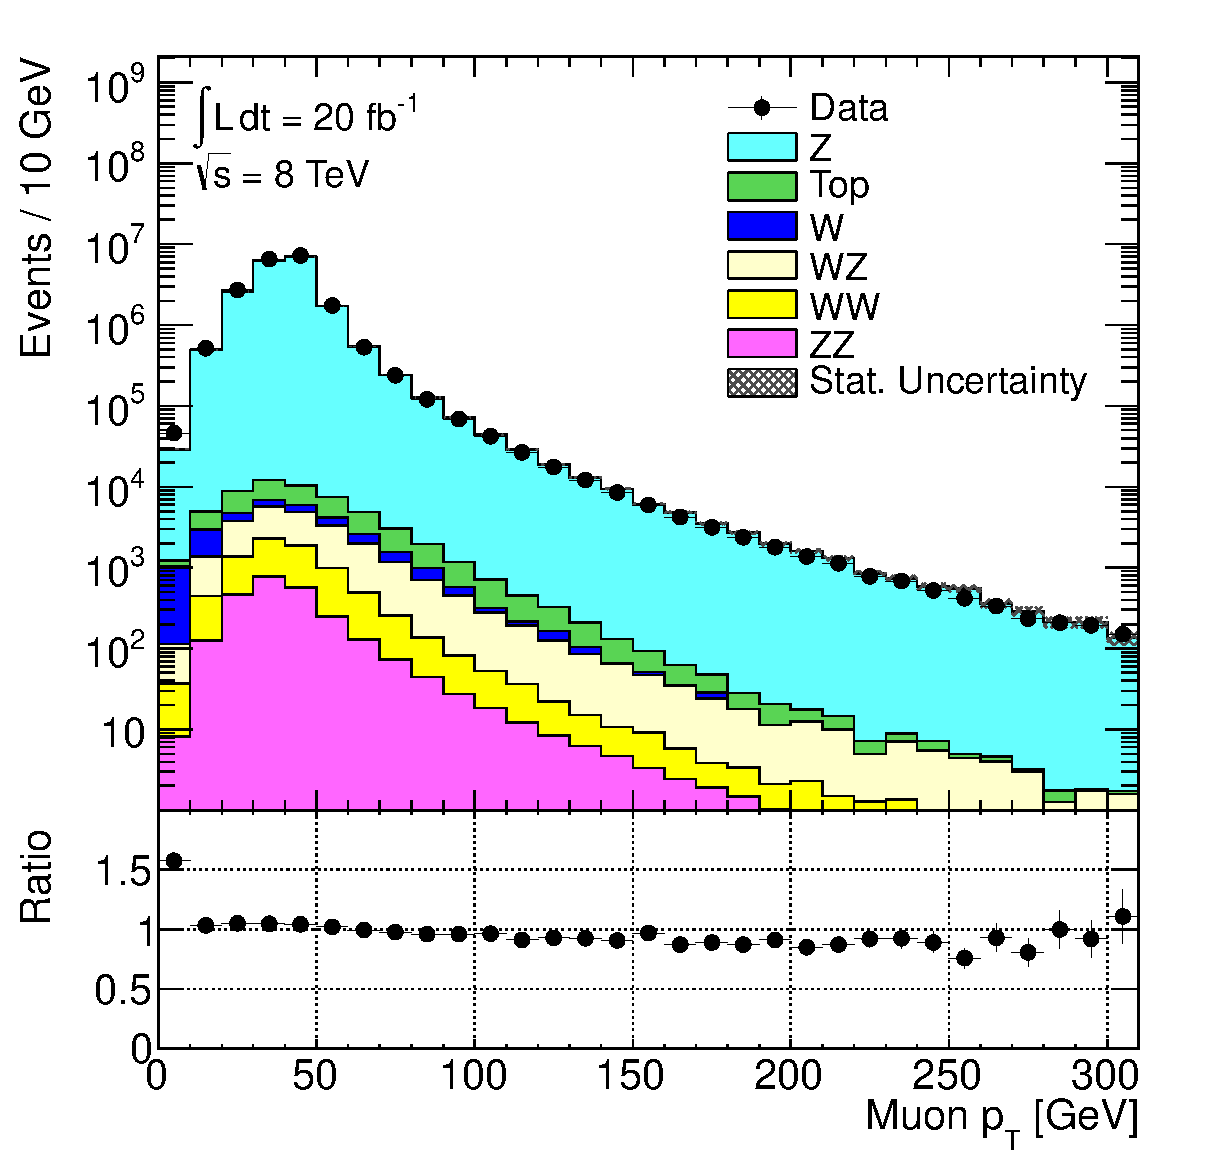
\includegraphics[width=0.47\textwidth]{Dilepton8TeVRatio/AllMu_lep_pt}
        }
	\subfigure[]{
            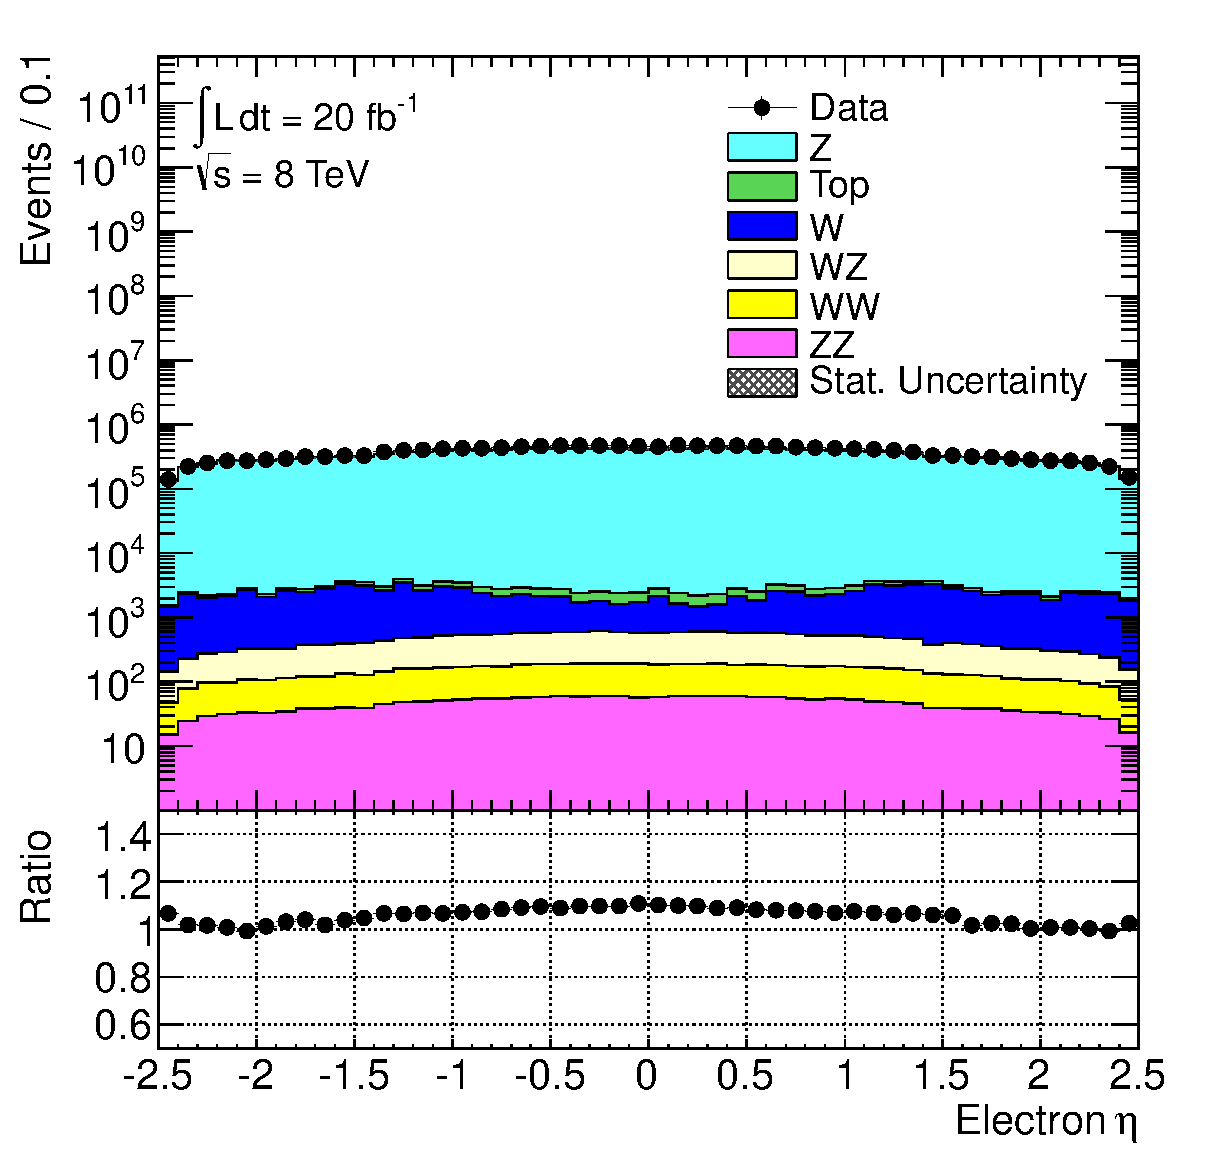
\includegraphics[width=0.47\textwidth]{Dilepton8TeVRatio/AllE_lep_eta}
        }
	\subfigure[]{
            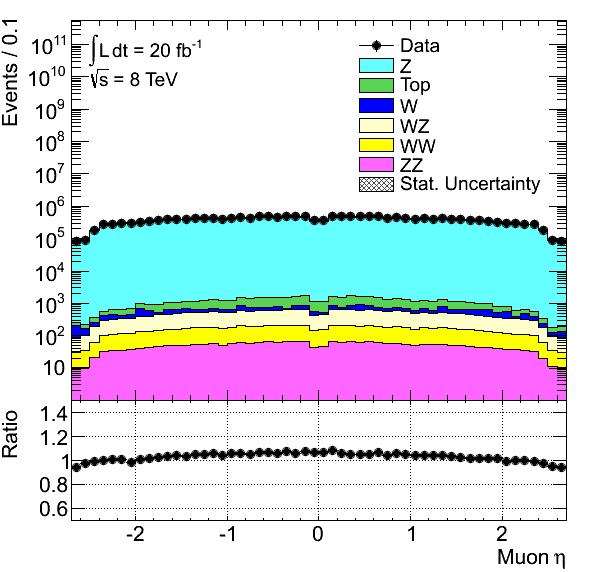
\includegraphics[width=0.47\textwidth]{Dilepton8TeVRatio/AllMu_lep_eta}
        }
	\subfigure[]{
            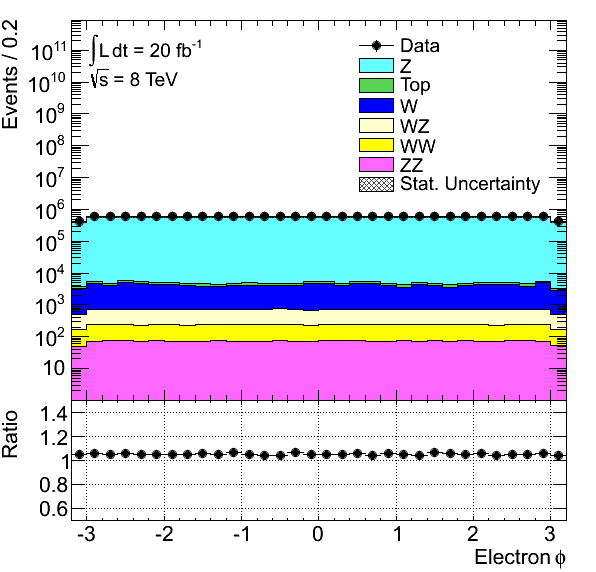
\includegraphics[width=0.47\textwidth]{Dilepton8TeVRatio/AllE_lep_phi}
        }
	\subfigure[]{
            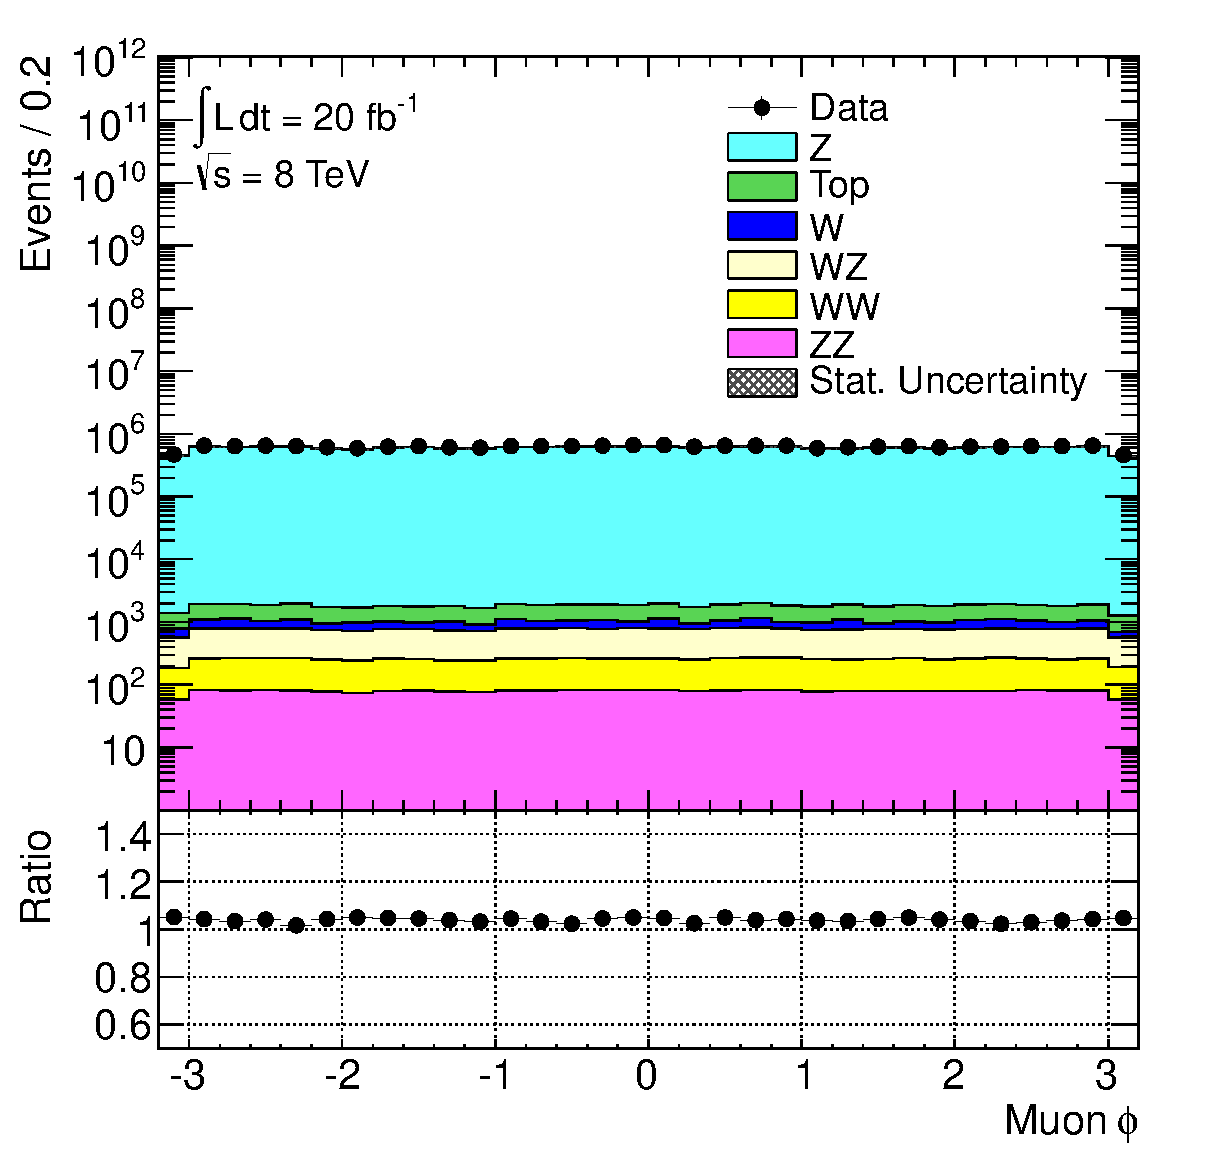
\includegraphics[width=0.47\textwidth]{Dilepton8TeVRatio/AllMu_lep_phi}
        }
    \caption[Lepton kinematic distributions for \dilep\ events in the 8~\tev\
    data. ]
    {\small Kinematic distributions for leptons in events in the 8~\tev\
    data containing an \ossf\ lepton pair. The leptons are required to pass all of the selection
    requirements described in Sections~\ref{sec:objsel-el}
    and~\ref{sec:objsel-mu} and the pair must have \sstooos. 
    Figures (a) and (b) show the lepton \pt\ for electrons and muons
    respectively, figures (c) and (d) the lepton $\eta$ and figures (d) and (e)
    the lepton $\phi$.    }
\label{fig:dilep-lepkin-eight}
\end{figure}

\begin{figure}[h]
\centering
	\subfigure[7~\tev]{
            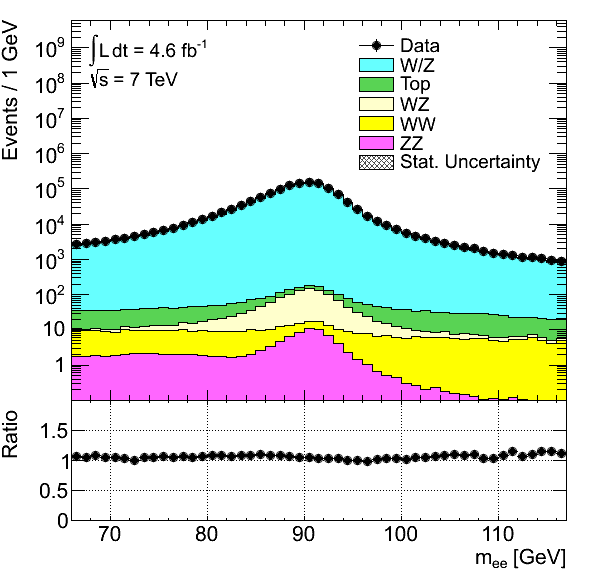
\includegraphics[width=0.47\textwidth]{Dilepton7TeVRatio/CeECeE_pt20MediumPP_Z_m}
        }
	\subfigure[8~\tev]{
            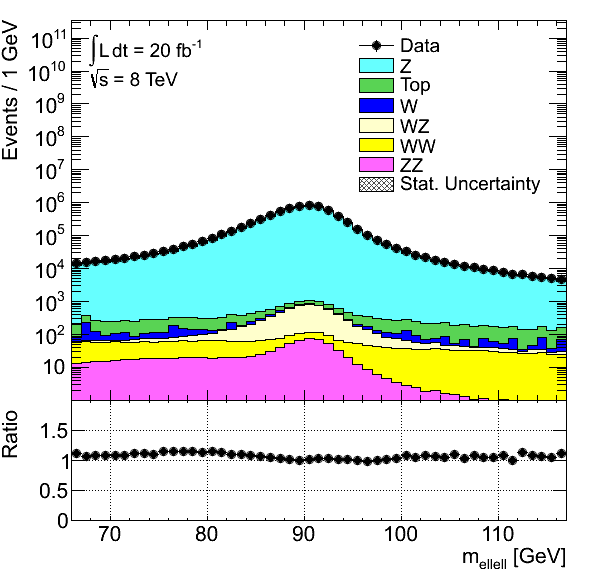
\includegraphics[width=0.47\textwidth]{Dilepton8TeVRatio/CeECeE_pt20MediumPP_Z_m}
        }
	\subfigure[7~\tev]{
            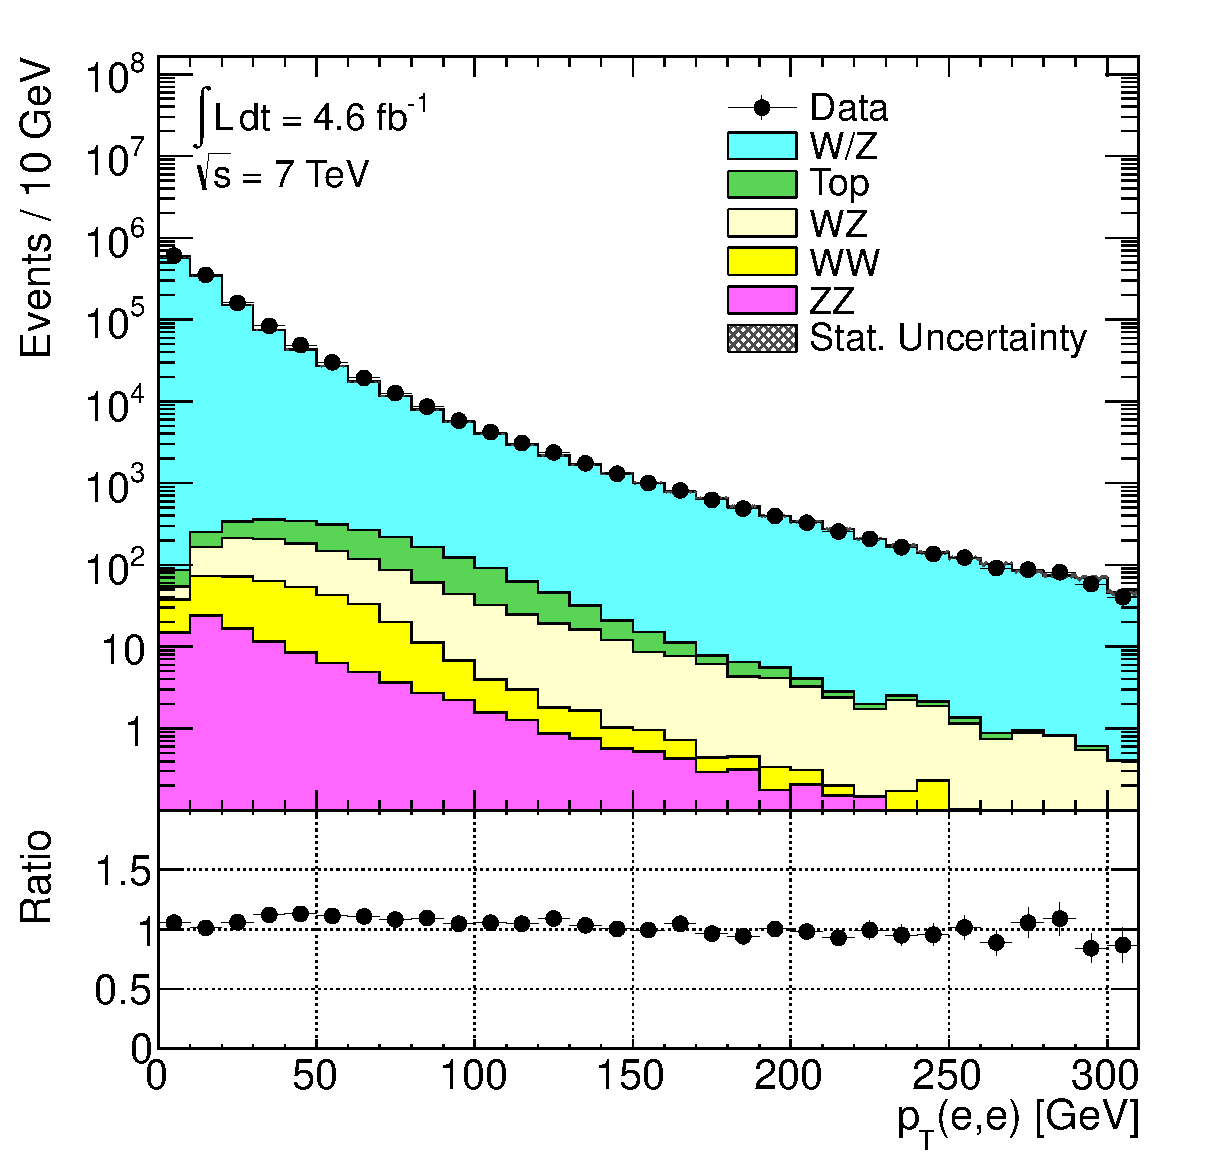
\includegraphics[width=0.47\textwidth]{Dilepton7TeVRatio/CeECeE_pt20MediumPP_Z_pt}
        }
	\subfigure[8~\tev]{
            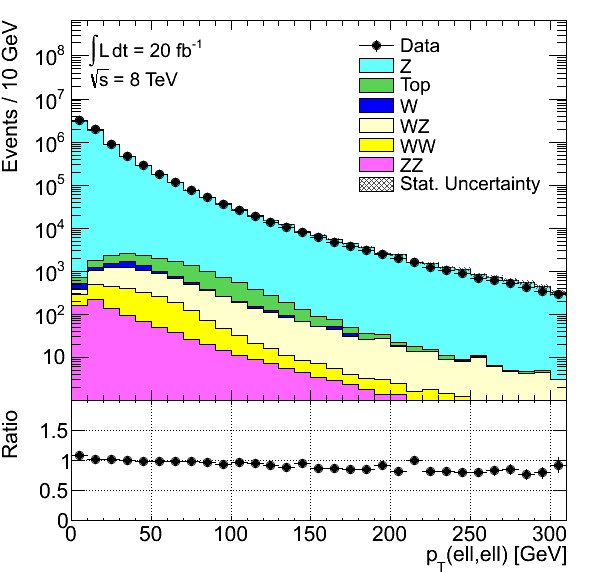
\includegraphics[width=0.47\textwidth]{Dilepton8TeVRatio/CeECeE_pt20MediumPP_Z_pt}
        }
    \caption[Dilepton invariant mass and transverse momentum in the 7~\tev\
    data. ]
    {Kinematic distributions for
    \dielectron\ pairs, for the 7~\tev\ and the 8~\tev\ data respectively, in events containing a pair of
    \ossf\ electrons with the electron selection tightened to require both
    electrons satisfy the \mediumPP\ requirements and have \ptgt{20}. 
    }
\label{fig:dilep-mass-pt-seven}
\end{figure}

\begin{figure}[h]
\centering
\vspace{-5mm}
	\subfigure[7~\tev]{
            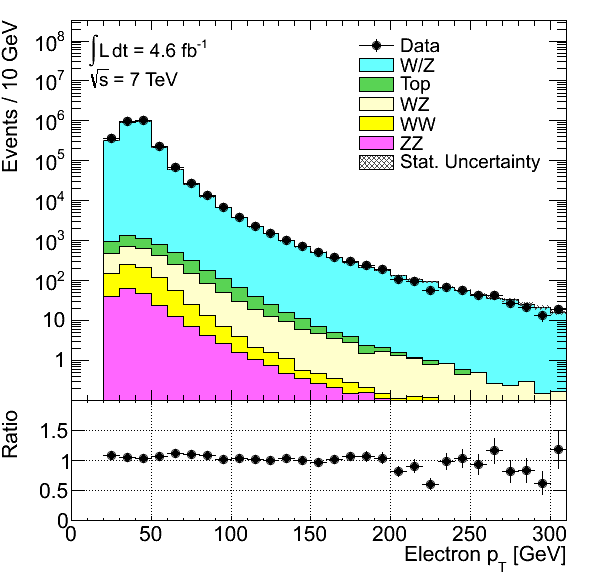
\includegraphics[width=0.47\textwidth]{Dilepton7TeVRatio/CeECeE_pt20MediumPP_lep_pt}
        }
	\subfigure[8~\tev]{
            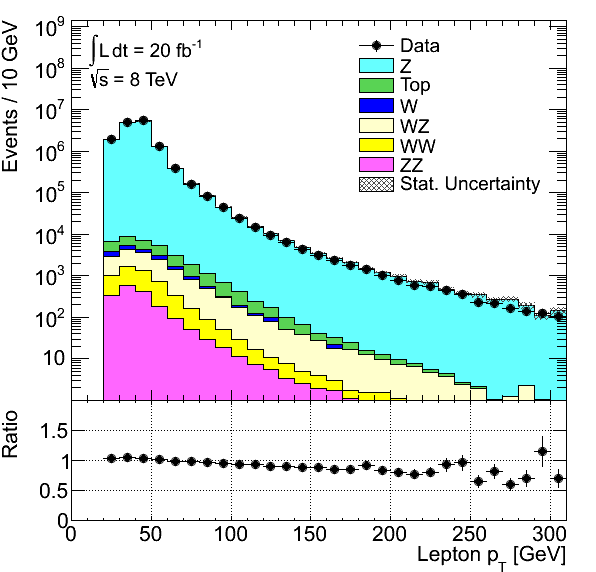
\includegraphics[width=0.47\textwidth]{Dilepton8TeVRatio/CeECeE_pt20MediumPP_lep_pt}
        }
	\subfigure[7~\tev]{
            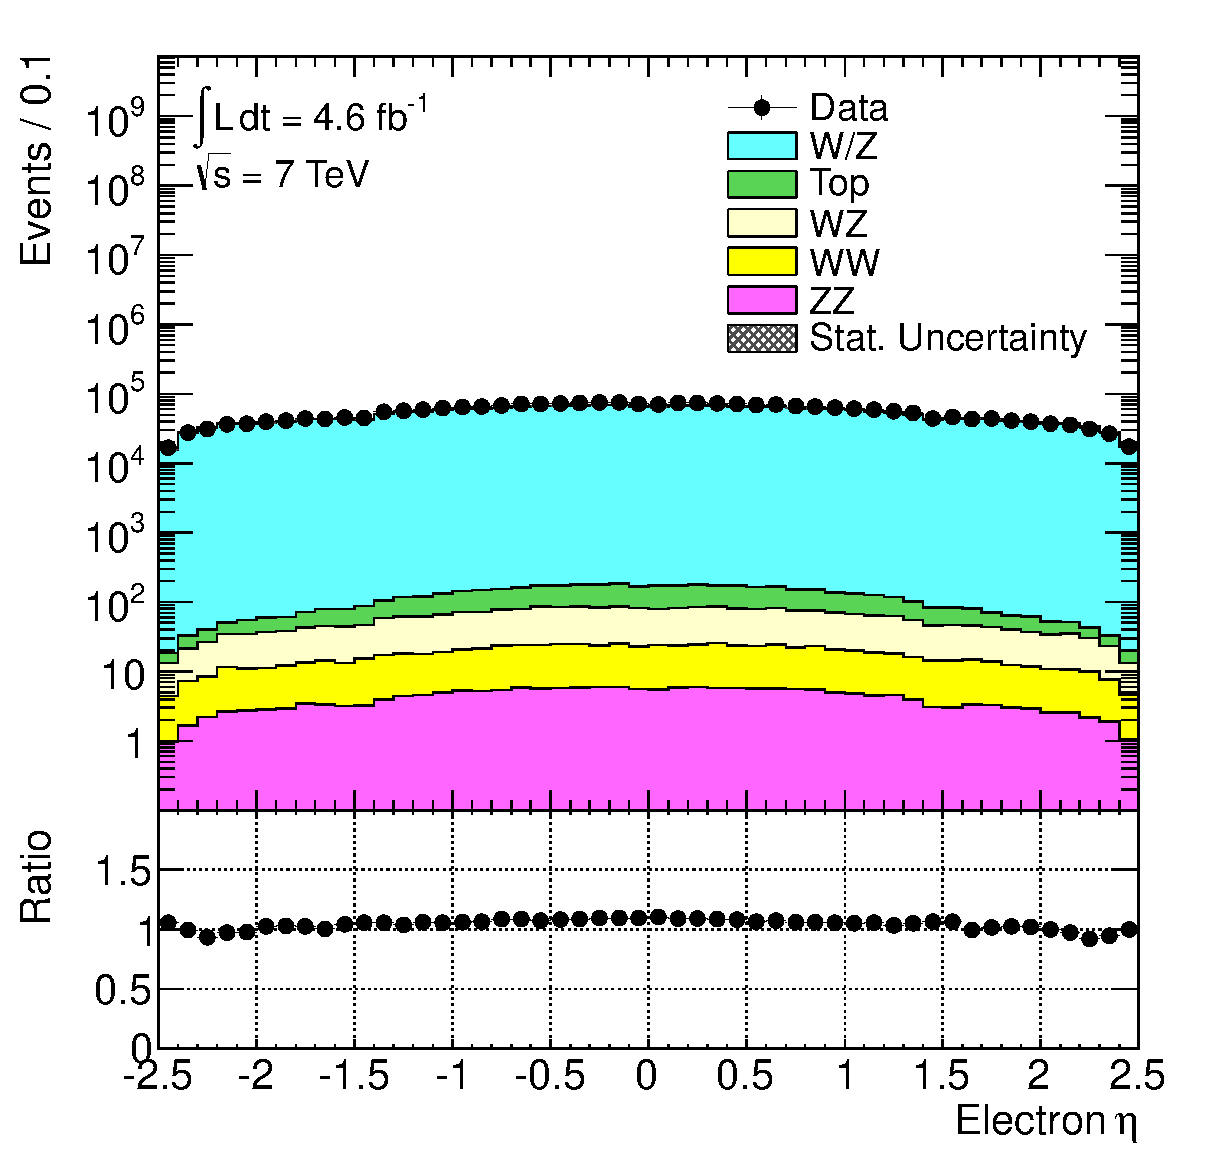
\includegraphics[width=0.47\textwidth]{Dilepton7TeVRatio/CeECeE_pt20MediumPP_lep_eta}
        }
	\subfigure[8~\tev]{
            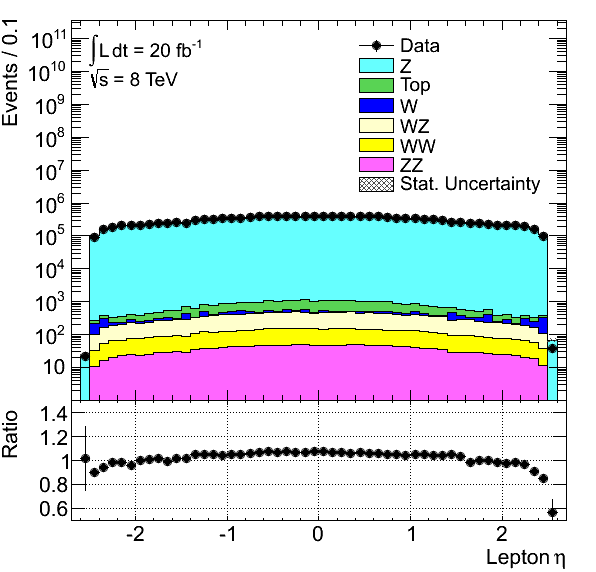
\includegraphics[width=0.47\textwidth]{Dilepton8TeVRatio/CeECeE_pt20MediumPP_lep_eta}
        }
	\subfigure[7~\tev]{
            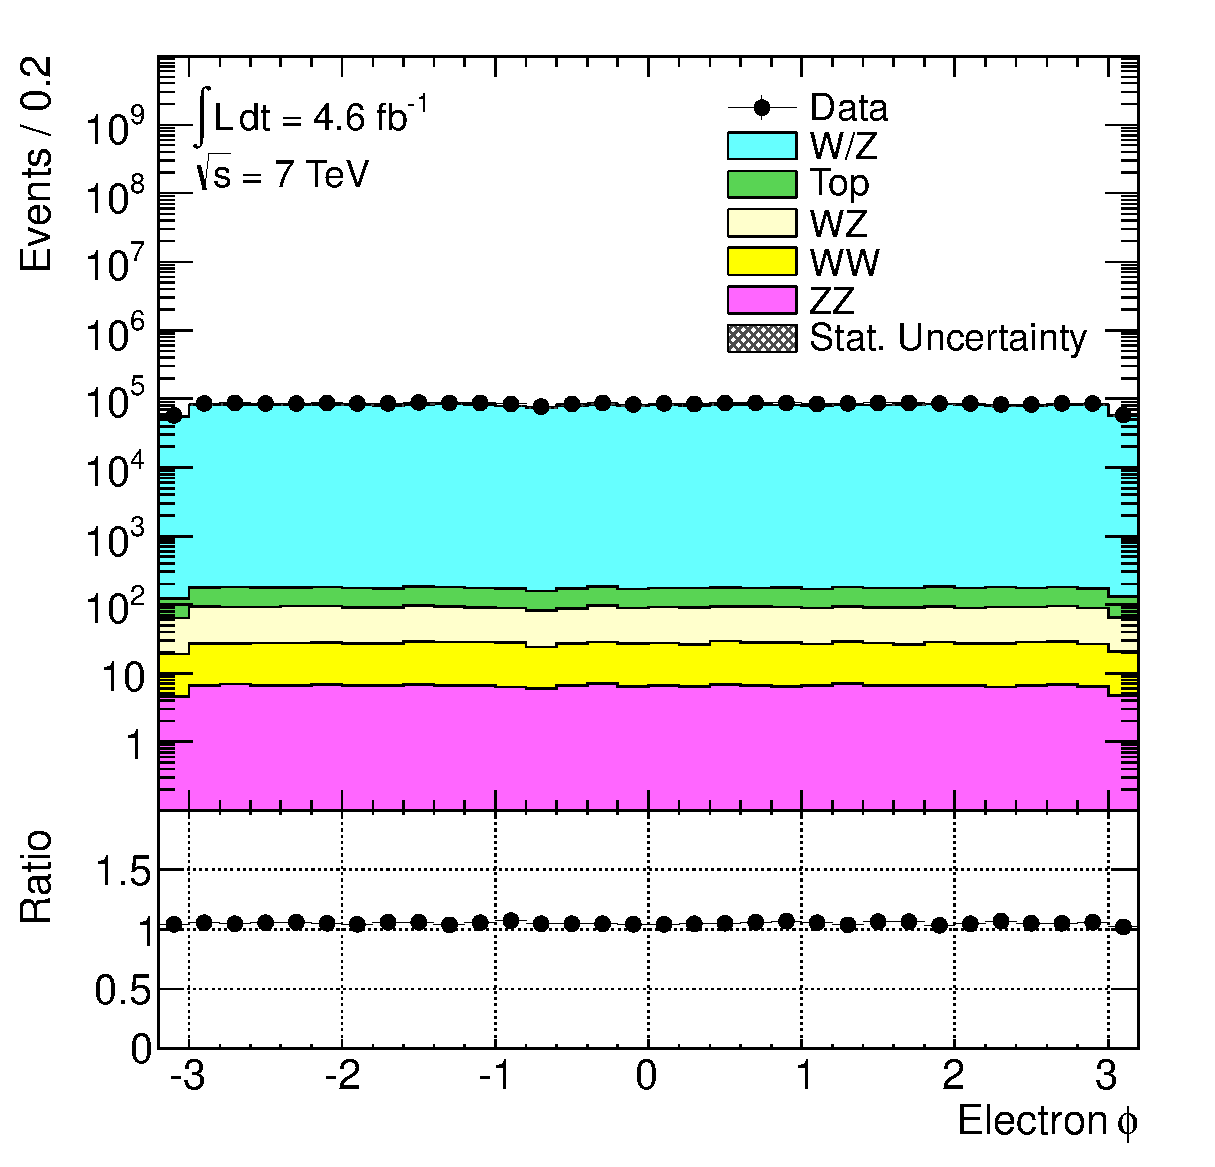
\includegraphics[width=0.47\textwidth]{Dilepton7TeVRatio/CeECeE_pt20MediumPP_lep_phi}
        }
	\subfigure[8~\tev]{
            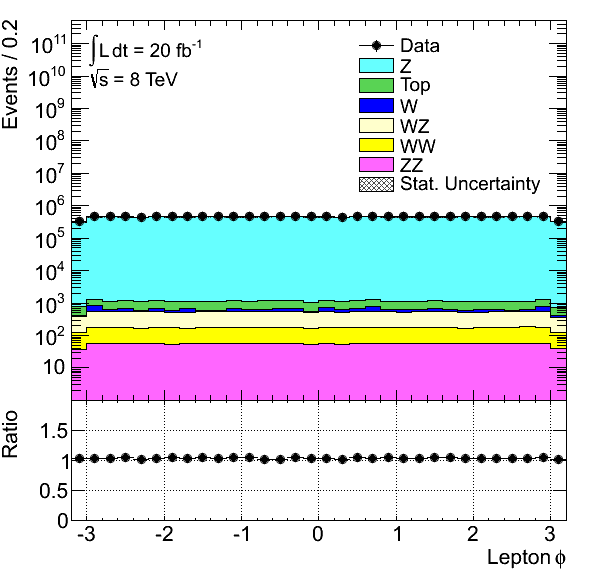
\includegraphics[width=0.47\textwidth]{Dilepton8TeVRatio/CeECeE_pt20MediumPP_lep_phi}
        }
    \caption[Lepton kinematic distributions for \dilep\ events in the 7~\tev\
    data. ]
    {\small Kinematic distributions for
    electron  in events containing a pair of
    \ossf\ electrons, with the electron selection tightened to require both
    electrons satisfy the \mediumPP\ requirements and have \ptgt{20}, for the 7~\tev\ and the 8~\tev\ data. }
\label{fig:dilep-lepkin-seven}
\end{figure}

\section{Increases from including `extension' leptons}

\begin{table}[htbp]
	 \centering
         \begin{tabular}{|l|ccc|c|}
         \hline\hline
         Object/channel & $4e$ & $2e2\mu$ &  $4\mu$ & $\ell\ell\ell\ell$\\\hline 
         High-Eta Muons               & $0.00$\% & $3.62$\% & $10.11$\% & $5.51$\% \\ 
         Calorimeter-tagged Muons     & $0.00$\% & $3.66$\% & $6.76$\% & $3.78$\% \\ 
         Both                         & $0.00$\% & $7.28$\% & $17.19$\% & $9.45$\% \\ 
         \hline\hline
	 \end{tabular}
	   \caption{Percentage increase in event yields for the 8~\tev\ analysis gained by extending the
           muon $\eta$ coverage from $|\eta|<2.5$ to  $|\eta|<2.7$ (``High-Eta Muons''), 
% by extending the electron $\eta$ coverage from $|\eta|<2.47$ to  $|\eta|<3.16$ (``Forward Electrons'') 
 and  by including calorimeter-tagged muons. The numbers are obtained from MC samples and apply after all \ZZ\ selection criteria. 
}
          \label{table:heta-muon-contribution}
\end{table}

\section{8~\tev\ Signal Plots with Irreducible Background}

\begin{figure}[htbp]
    \begin{center}
     \subfigure[]{
     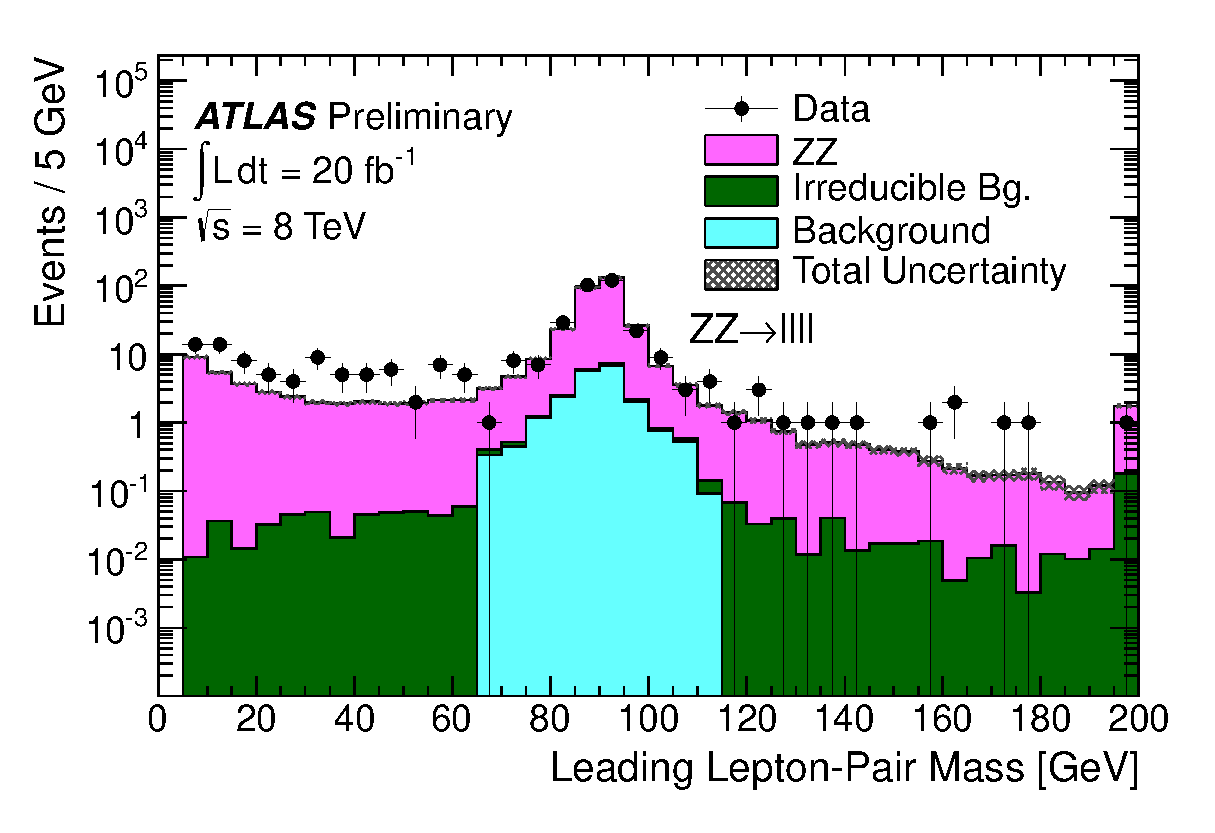
\includegraphics[width=0.47\textwidth]{SignalPlotsIrred/zMass1}
     }
     \subfigure[]{
     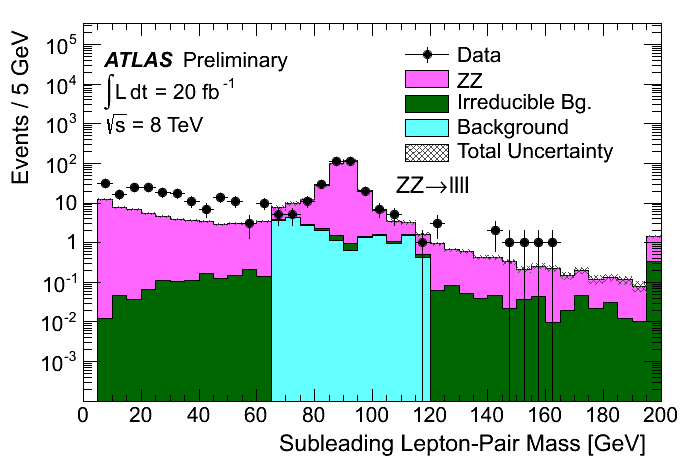
\includegraphics[width=0.47\textwidth]{SignalPlotsIrred/zMass2}
     }
     \subfigure[]{
     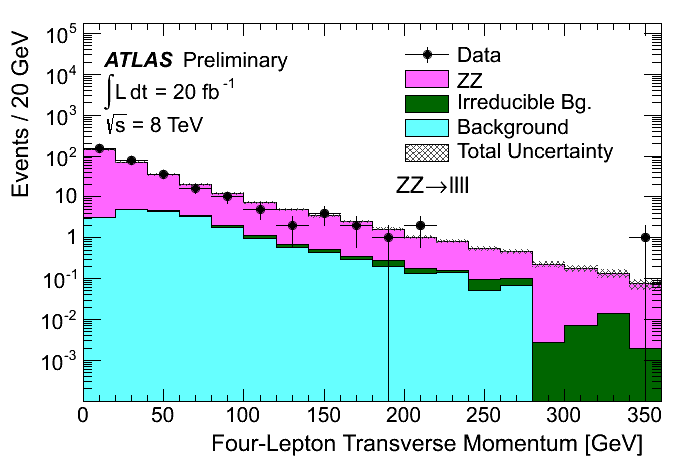
\includegraphics[width=0.47\textwidth]{SignalPlotsIrred/zzPt}
     }
     \subfigure[]{
     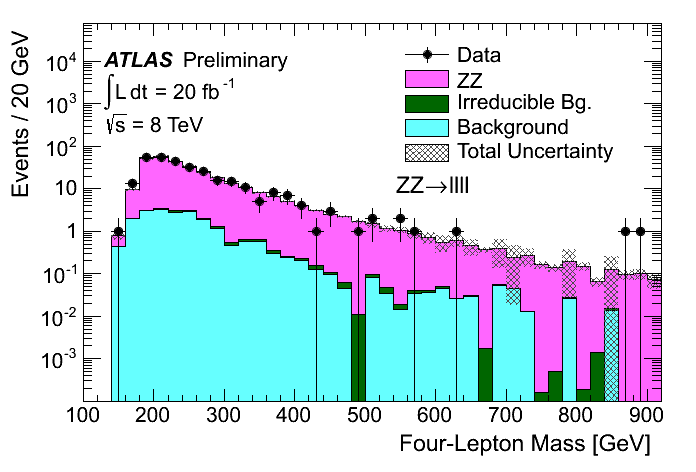
\includegraphics[width=0.47\textwidth]{SignalPlotsIrred/M4l}
     }
     \subfigure[]{
     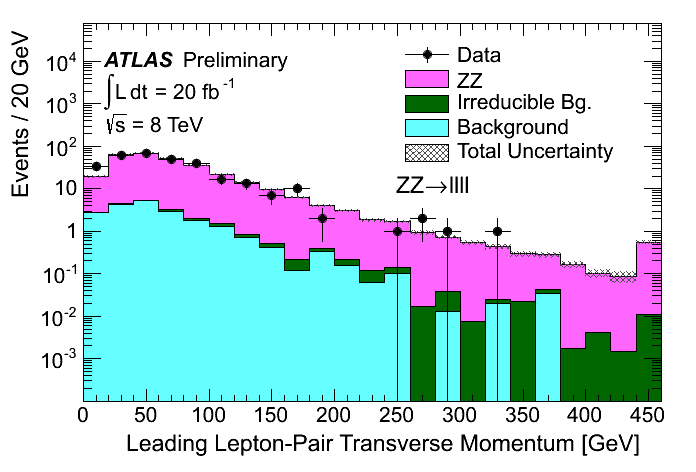
\includegraphics[width=0.47\textwidth]{SignalPlotsIrred/z1Pt}
     }
     \subfigure[]{
     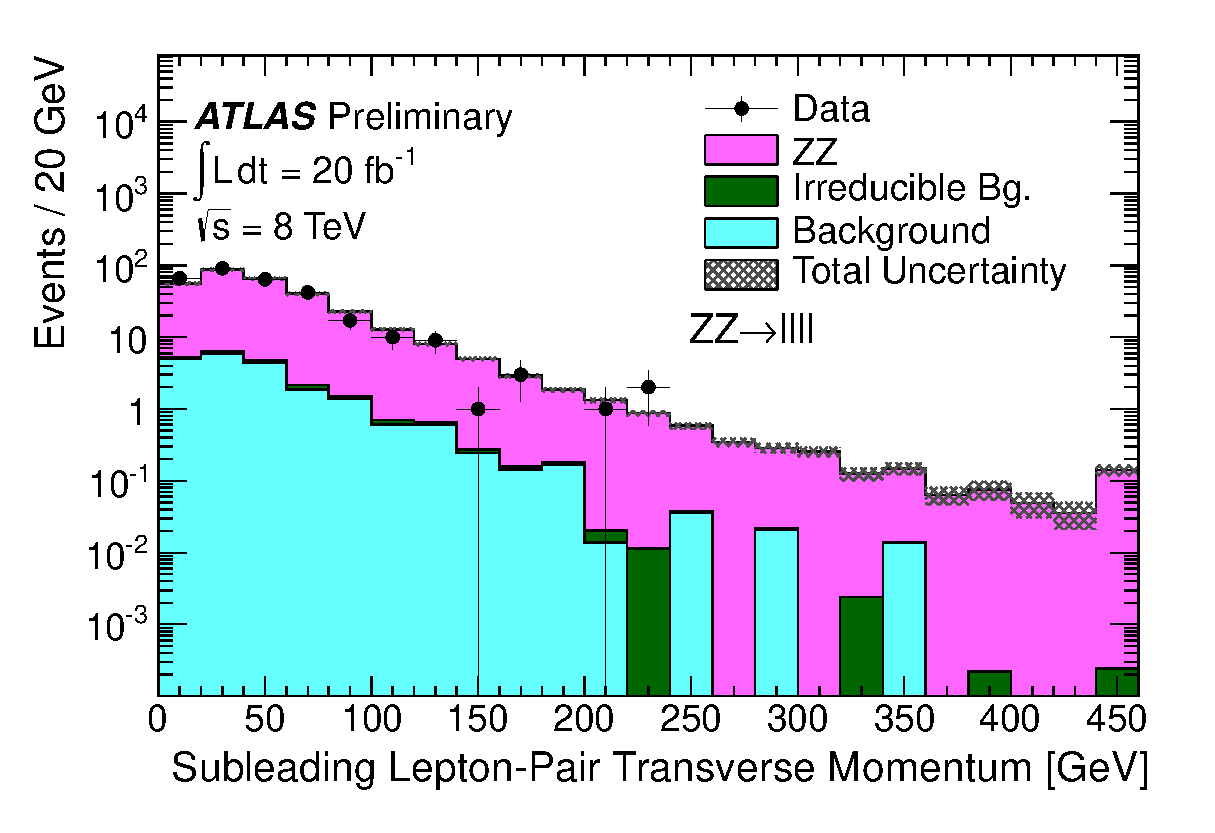
\includegraphics[width=0.47\textwidth]{SignalPlotsIrred/z2Pt}
     }
    \caption[Kinematic distributions for events passing the \ZZ\ selection in
    the 8~\tev\ data.]
    {Kinematic distributions for events passing the \ZZ\ selection in
    the 8~\tev\ data: (a) transverse momentum $\pT^{\ZZ}$ and (b) invariant mass $m^{\ZZ}$ of the 
    four-lepton system, (c) transverse momentum of the leading
    \dilep\ pair $\pt^{Z1}$, and (d) transverse momentum of the subleading
    \dilep\ pair $\pt^{Z2}$. The points represent the observed data and the pink histogram
    shows the prediction for the signal from simulation. The light blue
    histogram shows the background shape obtained from data, normalised to the
    total background estimate as described in~\chap{BackgroundEstimate}. The shaded band 
    shows the combined statistical and systematic uncertainty on the prediction. 
    }
    \label{fig:zzdists-ZZ-eight}
    \end{center}
\end{figure}
